\documentclass[UTF8]{ctexart}
\usepackage{fancyhdr}                                
\usepackage{lastpage}                                           
\usepackage{layout}  
\usepackage{amsmath}    
\usepackage{ragged2e} 
\usepackage{fancyhdr}                                
\usepackage{lastpage}                                           
\usepackage{layout}  
\usepackage{tikz}
\usepackage{amsmath}   
\usepackage{graphicx}        
\usepackage{subfigure}
\usepackage{listings}
\usepackage{bm}
\lstset{language=Matlab}
\lstset{breaklines}
\lstset{extendedchars=false}
\usepackage{array}
\usepackage{multirow}
\usepackage{booktabs}
\usepackage{caption}
\usepackage{paralist}
\usepackage{mathrsfs}
\usepackage{amsmath}
\usepackage{verbatim}
\usepackage{hyperref}
\usepackage{amsfonts}
\usepackage{algorithm}  
%\usepackage{algorithmic}
\usepackage{algorithm}
\usepackage{algpseudocode}  
\usepackage{graphicx}
\usepackage{float}
\usepackage{diagbox}    
\renewcommand\contentsname{Contents}                             
%\pagestyle{empty}                   %不设置页眉页脚        
\begin{document}
\title{\emph{Machine Learning: A Probabilistic Perspective} Solution Manual Version 2.1}
\author{Fangqi Li, Shanghai Jiao Tong University, P. R. China.}
\date{}
\maketitle
\tableofcontents
\newpage
\section{Preface: The Second Edition}
The tide of artificial intelligence (AI) has swept and reformed so many disciplines and pushed forward the borderline of the state-of-the-art. 
Such situation has resulted in a positive feedback that drives even more attention and effort into the study and research of AI, together with more unsettled regret and pities. 

I have participated in this study, with equal passion that any student who has not formed an exclusive view of the world should have when engaging in a booming subject. 
\begin{comment}
However, the reality has failed me by having unprincipled papers swarming in countless proceedings, capitals flowing not to those who are dying but those who are in charge of intelligent engineering whose only intelligence resides in the frontpage of their documentations, eager students and scholar looking for sponsorships struggling for hybridizing frail theories and intractable demands. 
Those deeds make a mockery of what AI and machine learning (ML) should have been. 
What made the situation more miserable is that I, though have been overlooking those facts, have deeply involved and even evoked more of them. 
For this reason I decided to put forward my understanding of AI/ML, to which myself fail to insist from time to time, in a prudent way at the begining of this document. 

To my view, ML is nothing more than applying statistics to estimate and infer. 
For tasks where a compact formulation is readily available, an ideal solution can be obtained by yielding computational resources, as what has been deduced ages before. 
For those whose formulation itself is vague, controversial and empirically out of the scope of a fair discussion whose language could have gone beyond the intercourse of human reasons,  I do not expect any plausible outcomes from artificial intelligence. 

To challenge and despise those working with relatively traditional disciplines is what many students engaging in ML, at least some part of me, loves to, or what has boosted their efforts. 
But it turns out that despite of some innovations that have been predicted centuries ago, the advantages that AI and ML have brought is not charming enough as some scholars have claimed, be it ever charming for someone. 
The studies of ML should be dedicated to the expanison of the range of merits for human being and the elimination of injustice and partiality, as is any engineering subject. 
But actually they have done so so few, or at least fewer than I have once imaged. 

I made the argument above in the hope of reminding any potential reader of the limit of AI, the reason behind is three-folded:
\begin{itemize}
\item The other direction of this line, in which a student might learn the capability of AI and ML, or practical Bayesian statistics, and become a confident, reliable engineer is being shed light on in the textbook whose solution manual is going to be presented. 
I believed that any reader of this document has been substantially motivated in this direction. 
Thus I thought that some voices from the other side could be helpful, even for the naive reason of balance. 
\item I tried to embed the apprehension and pity for the suffering of mankind in a reader's mind, after which she/he can form a modest and stoic view of AI, which is believed to be the cornerstone of the revolution of industry, epistemology, and the society.
I do not that this embedding can last for long, but without these discourses of embedding the influence that I would like to exert could only be weaker. 
This is what I have been experiencing when I pursued a degree of art in the university. 
Though I am currently working toward a degree of science and engineering, this apprehension is what I recognized to be the most important for a scholar, or one who is becoming a scholar, or a decent human, at length.
\item I am standing in a position where anxiety and tranquilness keep reminding me of my incompetence and cowardice night after night. 
It is these evenings that challenge my belief in the subject which I have tangled and had delight with, and force me to reckon the limits of my knowledge. 
I believed that some readers, be their number so negligible, could be confronted with the similar hopeless nights in one day. 
I know not how to allievate this suffer, but I hope the fact that they are not experiencing these miseries alone could illuminate their paths across these restless evenings. 
Those are words that I have wished to hear, for which reason I speak it out. 
\end{itemize} 
\end{comment}

It has been three years and four months since I started the first edition of this solution manual. 
Although I have received no patron and have no intention of finding one, I received several grateful and advisory messages, from which I felt more pleased than having any of my technical papers published online. 
For the convenience of them, I would gladly edit this manuscript again, be the time goes back to 2017. 
In the second edition, I tried to be more concrete in deduction so readers can follow up easier. 
Some graphical or numerical examples were provided to increase the overall readability. 
The purpose of this manuscript is, as its first edition, to complete the textbook \emph{Machine Learning, A Probabilistic Perspective} as a closed collection of knowledge as far as I could, and to save those who are lost in the ocean of deduction and symbols in ML, whom any talent mind could have become for some times in his/her course with this textbook. 
I hope that this manuscript can help, be it ever so little, to any reader who purposedly or accidently finds it. 

I personally take responsibility for any typo, or mistake in $\beta$-reductions. 

Fangqi Li,

Shanghai Jiao Tong University,

Shanghai, P.R.China.

January the 4th, 2021.

Contact me by: \url{solour_lfq@sjtu.edu.cn} or \url{1524587011@qq.com}.

My homepage is at: \url{https://solour-lfq.github.io/}.

\newpage
\centerline{\Large{第二版序}}

这篇文档的主体由英文书写,这一方面是因为英文是学术上最泛用的语言,有利于本文档的传播;另一方面是我认为有能力阅读MLaPP原教材的中国学生、汉语母语学生基本上也能畅通无阻地阅读本文档中的英文。

希望中国学者和其他可以以中文为语言写作的学者一同努力,提升中文期刊、会议的质量和中文区科研院所的硬实力、影响力,让越来越多的学者乐于用中文叙述自己的观点。

第二版修订了第一版的一些文本问题,补充了第一版在习题推理上比较缺少的理念连接,同时增加了一些示例以提升可读性。文档内的所有排版错误、推导错误由我一人负责。

李方圻

上海交通大学

2021年1月4日

邮箱:\url{solour_lfq@sjtu.edu.cn},\url{1524587011@qq.com}。

主页:\url{https://solour-lfq.github.io/}。

\newpage
\section{Introduction (Preface of the First Edition)}
\subsection{Constitution of this document}
Here we should have demonstrated the solution to problems in Chapter One in \emph{Machine Learning, A Probabilistic Perspective}(MLAPP). Since the number of problem in Chapter is zero, we save this section as an introduction to this document, i.e.a solution manual.

This document provides detailed solution to almost all problems of textbook MLAPP from Chapter One to Chapter Fourteen(Chinese version) / Twenty-one(English version). We generally save the restatement of problems for readers themselves. 

There are two class for problems in MLAPP: theortical inference and pratical projects. We provide solution to most inference problems apart from those which are nothing but straightforward algebra(and few which we failed to solve). Practical problems, which base on a Matlab toolbox, are beyond the scope of this document.

\subsection{On \emph{Machine Learning: A Probabilistic Perspective}}
Booming studies and literatures have made the boundary of "machine learning" vague.

On one hand, the rapid development of AI technology has kept the society shocked, which also results in sharply increase in number of students who would try to take related courses in colleges. On the other hand, some scholars are still uncertain in learning-related theories, especially deep learning.

The extraordinary achievements of machine learning in recent days often make one forget that this discipline has undergone a long evolution and whose establishment dates back at least to the studies of "electronic brains" in the 1940s. Be that as it may, machine learning has not been defined as a "closed" theory. Even in the some community of researchers, machine learning are crowned metaphysics or alchemistry. Personally, I believe tha being called metaphysics is a common experience shared by many branches of theory which are undergoing the most rapid development.

To be a completed theory, machine learning is still looking for a way to conclude itself in a closed system. The most successful attempt so far has been the one based on probability. As commented by David Blei from Princton on the back of MLAPP: "In Machine Learning, the language of probability and statistics reveals important connections between seemingly disparate algorithms and strategies. Thus, its readers will become articulate in a holistic view of the state-of-art and poised to build the next generation of machine learning algorithms."

The crucial idea in MLAPP is: machine learning is tantamount to Bayesian Statistics, which draws connections between numerous "indepedent" algorithms. But the history of Bayesian statistics(which can be traced back to days of Laplace) outlengths the one of machinea learning a lot. MLAPP is not noval in holding such an idea. C.M.Bishop's \emph{Pattern Recognition and Machine Learning} is another typical example. Both of them are considered as classical textbooks in elementary machine learning.

In general, MLAPP reduces the difficulty of the entire book at the expense of partially deduced completeness(for the first seven chapters). It covers a wider range of models and is suitable for those with background in mathemathcal tools. The chapters that concerning classical probabilistic models (e.g, chapter 2, 3, 4, 5, 7, 8, 11, 12) is comparable to PRML. But due to the reordering and more details, they worth a read for one who have finished reading PRML. 

\subsection{What is this document?}
The motivation for writing this document is that I need to read textbook MLAPP after selecting machine learning course, but I failed to find any free compiled solution manuals. Although several Github projects have started working on it, the velocity has been too slow. Also I want to focus more on the theoretical part of the text rather than the implementation code.

Hence I began working on this document. It is completed(first version, Chapter One to Chapter Fourteen) within the first two weeks before the official semester. Bacase of the hurry process, it is suggested that readers should read from a critical perspective and not hesitate to believe in everything I have written down. In the end, I hope that readers can provide comments and revise opinions. Apart from correcting the wrong answers, those who good at using MATLAB, Latex typesetting or those who are willing to participate in the improvement of the document are always welcome to contact me.

\ 

\ 

\ 

22/10/2017

Fangqi Li

Munich, Germany

\url{solour_lfq@sjtu.edu.cn}

\url{ge72bug@tum.de}

\newpage
\subsection{Updating log}
22/10/2017(First Chinese compilation)

02/03/2018(English compilation)


\newpage
\section{Probability}
\subsection{Probability are sensitive to the form of the question that was used to generate the answer}
Denote two children by $A$ and $B$.

Use 
$$E_{1}:A=boy,B=girl$$
$$E_{2}:B=boy,A=girl$$
$$E_{3}:A=boy,B=boy$$

In question a:

$$P(E_{1})=P(E_{2})=P(E_{3})=\frac{1}{4}$$

$$P(OneGirl|OneBoy)=\frac{P(E_{1})+P(E_{2})}{P(E_{1})+P(E_{2})+P(E_{3})}=\frac{2}{3}$$

For question b,w.l.o.g, assume child $A$ is seen:
$$P(B=girl|A=boy)=\frac{1}{2}$$

\subsection{Legal reasoning}
Let $E_{1}$ and $E_{2}$ denote the event "the defendant commited the crime" and "the defendant has special blood type" respectively. Thus:
\begin{align}
p(E_{1}|E_{2})=&\frac{p(E_{1},E_{2})}{p(E_{2})}=\frac{p(E_{2}|E_{1})p(E_{1})}{p(E_{2})} \nonumber \\
=&\frac{1\cdot \frac{1}{800000}}{\frac{1}{8000}}=\frac{1}{100} \nonumber
\end{align}

\subsection{Vriance of a sum}
Calculate this straightforwardly:
\begin{align}
var[X+Y]=&\mathbb{E}[(X+Y)^{2}]-\mathbb{E}^{2}[X+Y] \nonumber \\
=&\mathbb{E}[X^{2}]-\mathbb{E}^{2}[X]+\mathbb{E}[Y^{2}]-\mathbb{E}^{2}[Y]+2\mathbb{E}[XY]-2\mathbb{E}^{2}[XY] \nonumber \\
=&var[X]+var[Y]+2cov[X,Y]\nonumber
\end{align}

\subsection{Bayes rule for medical diagnosis}
Applying Bayes's rules:
\begin{align}
P(ill|positive)=&\frac{P(ill)P(positive|ill)}{P(ill)P(positive|ill)+P(health)P(positive|health)} \nonumber \\
=&0.0098 \nonumber
\end{align}

\subsection{The Monty Hall problem(The dilemma of three doors)}
The answer is b. Applying Bayes's rules:
\begin{align}
P(prize_{1}|choose_{1},open_{3})=&\frac{P(choose_{1})P(prize_{1})P(choose_{3}|prize_{1},choose_{1})}{P(choose_{1})P(open_{3}|choose_{1})}\nonumber \\
=&\frac{P(prize_{1})P(choose_{3}|prize_{1},choose_{1})}{P(open_{3}|choose_{1})}\nonumber \\
=&\frac{\frac{1}{3}\cdot\frac{1}{2}}{\frac{1}{3}\cdot \frac{1}{2} + \frac{1}{3}\cdot 0 + \frac{1}{3} \cdot 1}=\frac{1}{3} \nonumber
\end{align}

In the last step we summarize over the potential location of the prize.

\subsection{Conditional Independence}
In question a, we have:
$$p(H|e_{1},e_{2})=\frac{p(H)p(e_{1},e_{2}|H)}{p(e_{1},e_{2})}$$

Thus the answer is (ii).

For question, we have further decomposition:
$$p(H|e_{1},e_{2})=\frac{p(H)p(e_{1}|H)p(e_{2}|H)}{p(e_{1},e_{2})}$$

So both (i) and (ii) and sufficient obviously. Since:
\begin{align}
p(e_{1},e_{2})=& \sum_{H}p(e_{1},e_{2},H) \nonumber \\
=&\sum_{H} p(H)p(e_{1}|H)p(e_{2}|H) \nonumber 
\end{align}

(iii) is sufficint as well since we can calculate $p(e_{1},e_{2})$ independently.

\subsection{Pairwise independence does not imply mutual independence}
Let's assmue three boolean variables $x_{1},x_{2},x_{3}$, $x_{1}$ and $x_{2}$ have values of 0 or 1 with equal possibility independently and $x_{3}=XOR(x_{1},x_{2})$:

It is easy to prove that $x_{3}$ is independent with $x_{1}$ or $x_{2}$, but given both $x_{1}$ and $x_{2}$, the value of $x_{3}$ is determined and thereby the mutual independence fails.

\subsection{Conditional independence iff joint factorizes}
We prove 2.129 is equal to 2.130.

By denoting:
$$g(x,z)=p(x|z)$$
$$h(y,z)=p(y|z)$$

We have the first half of proof.

Secondly we have:
\begin{align}
p(x|z)=&\sum_{y}p(x,y|z) \nonumber \\
=&\sum_{y}g(x,z)h(y,z) \nonumber \\
=&g(x,z)\sum_{y}h(y,z) \nonumber \\
p(y|z)=&h(y,z)\sum_{x}g(x,z_)\nonumber 
\end{align}

And:
\begin{align}
1=&\sum_{x,y}p(x,y|z) \nonumber \\
=&(\sum_{x}g(x,z))(\sum_{y}h(y,z)) \nonumber
\end{align}

Thus:
\begin{align}
p(x|z)p(y|z)=&g(x,z)h(y,z)(\sum_{x}g(x,z))(\sum_{y}h(y,z)) \nonumber \\
=&g(x,z)h(y,z) \nonumber \\
=&p(x,y|z) \nonumber
\end{align}

\subsection{Conditional independence*}
From a graphic view, both arguments are correct. But from a general view, both of them do not have a decomposition form, thus false.

\subsection{Deriving the inverse gamma density}
According to:
$$p(y)=p(x)|\frac{dx}{dy}|$$

We easily have:
\begin{align}
IG(y)=&Ga(x)\cdot y^{-2} \nonumber \\
=&\frac{b^{a}}{\Gamma(a)}(\frac{1}{y})^{(a-1)+2}e^{-\frac{b}{y}} \nonumber \\
=&\frac{b^{a}}{\Gamma(a)}(y)^{-(a+1)}e^{-\frac{b}{y}} \nonumber
\end{align}

\subsection{Normalization constant for a 1D Gaussian}
This proof should be found around any textbook about multivariable calculus.Omitted here.

\subsection{Expressing mutual information in terms of entropies}
\begin{align}
I(X;Y)=&\sum_{x,y}p(x,y) \log \frac{p(x,y)}{p(x)p(y)} \nonumber \\
=&\sum_{x,y}p(x,y)\log \frac{p(x|y)}{p(x)} \nonumber \\
=&\sum_{x,y}p(x,y)\log p(x|y) - \sum_{x}(\sum_{y}p(x,y))\log p(x) \nonumber \\
=&-H(X|Y)+H(X) \nonumber
\end{align}

Inversing $X$ and $Y$ yields to another formula..

\subsection{Mutual information for correlated normals}
We have:
\begin{align}
I(X_{1};X_{2})=&H(X_{1})-H(X_{1}|X_{2}) \nonumber \\
=&H(X_{1})+H(X_{2})-H(X_{1},X_{2}) \nonumber \\
=&\frac{1}{2}\log 2\pi\sigma^{2}+\frac{1}{2}\log 2\pi\sigma^{2}+\frac{1}{2}\log (2\pi)^{2}\sigma^{4}(1-\rho^{2}) \nonumber \\
=&-\frac{1}{2}\log (1-\rho^{2}) \nonumber
\end{align}

(refer to \textbf{Elements of Information Theory},Example 8.5.1)

\subsection{A measure of correlation}
In question a:
\begin{align}
r=&1-\frac{H(Y|X)}{H(X)}=\frac{H(X)-H(Y|X)}{H(X)} \nonumber \\
=&\frac{H(Y)-H(Y|X)}{H(X)} \nonumber \\
=&\frac{I(X;Y)}{H(X)} \nonumber 
\end{align}

We have $0 \leq r \leq 1$ in question b for $I(X;Y) > 0$ and $H(X|Y) < H(X)$(properties of entropy).

$r=0$ iff $X$ and $Y$ are independent.

$r=1$ iff $X$ is determined(not necassary equal) by $Y$.

\subsection{MLE minimizes KL divergence to the empirical distribution}
Expand the KL divergence:
\begin{align}
\theta=&\arg\min_{\theta}\left\{ \mathbb{KL}(p_{emp}||q(\theta)) \right\} \nonumber \\
=&\arg\min_{\theta}\left\{ \mathbb{E}_{p_{emp}}[\log \frac{p_{emp}}{p(\theta)}] \right\} \nonumber \\
=&\arg\min_{\theta}\left\{ -H(p_{emp}) - \sum_{\textbf{x}\in dataset}(\log q(\textbf{x};\theta)) \right\} \nonumber \\
=&\arg\max_{\theta}\left\{ \sum_{\textbf{x}\in dataset} \log p(\textbf{x};\theta)\right\} \nonumber
\end{align}
 
We use the weak law of large numbers in the third step and drop the entropy of empirical distribution in the last step.

\subsection{Mean, mode, variance for the beta distribution}
Firstly, derive the mode for beta distribution by differentiating the pdf:
$$\frac{d}{dx}x^{a-1}(1-x)^{b-1}=[(1-x)(a-1)-(b-1)x]x^{a-2}(1-x)^{b-2}$$

Setting this to zero yields:
$$mode=\frac{a-1}{a+b-2}$$

Secondly, derive the moment in beta distribution:
\begin{align}
\mathbb{E}[x^{N}]=&\frac{1}{B(a,b)}\int x^{a+N-1}(1-x)^{b-1} dx \nonumber \\
=&\frac{B(a+N,b)}{B(a,b)} \nonumber \\
=&\frac{\Gamma(a+N)\Gamma(b)}{\Gamma(a+N+b)} \frac{\Gamma(a+b)}{\Gamma(a)\Gamma(b)} \nonumber 
\end{align}

Setting $N=1,2$:
$$\mathbb{E}[x]=\frac{a}{a+b}$$
$$\mathbb{E}[x^{2}]=\frac{a(a+1)}{(a+b)(a+b+1)}$$

Where we have used the property of Gamma function. Straightforward algebra gives:
$$mean=\mathbb{E}[x]=\frac{a}{a+b}$$
$$variance=\mathbb{E}[x^{2}]-\mathbb{E}^{2}[x]=\frac{ab}{(a+b)^{2}(a+b+1)}$$

\subsection{Expected value of the minimum}
Let $m$ denote the location of the left most point, we have:
\begin{align}
p(m>x)=&p([X>x] \textbf{and} [Y>x])\nonumber \\
=&p(X>x)p(Y>x) \nonumber \\
=&(1-x)^{2} \nonumber
\end{align}

Therefore:
\begin{align}
\mathbb{E}[m]=&\int x\cdot p(m=x)dx \nonumber \\
=&\int p(m>x)dx \nonumber \\
=&\int_{0}^{1}(1-x)^{2}dx \nonumber \\
=&\frac{1}{3}\nonumber
\end{align}

\newpage
\section{Generative models for discrete data}
\subsection{MLE for the Beroulli/binomial model}
Likelihood:
$$p(D|\theta) = \theta^{N_{1}}(1-\theta)^{N_{0}}$$

Log-Likelihood:
$$\ln p(D|\theta) = N_{1}\ln \theta + N_{0} \ln (1-\theta)$$

Setting the derivative to zero:
$$\frac{\partial}{\partial \theta} \ln p(D|\theta) = \frac{N_{1}}{\theta} -\frac{N_{0}}{1-\theta}=0$$

This ends in 3.22:
$$\theta = \frac{N_{1}}{N_{1}+N_{0}}=\frac{N_{1}}{N}$$

\subsection{Marginal likelihood for the Beta-Bernoulli model}
Likelihood:
$$p(D|\theta) = \theta^{N_{1}}(1-\theta)^{N_{0}}$$

Prior distribution:
$$p(\theta|a,b)=Beta(\theta|a,b)=\theta^{a-1}(1-\theta)^{b-1}$$

Posterior distribution:
\begin{align}
p(\theta|D) \propto& p(D|\theta)\cdot p(\theta|a,b)\nonumber \\
=&\theta^{N_{1}+a-1}(1-\theta)^{N_{0}+b-1}\nonumber \\
=&Beta(\theta|N_{1}+a,N_{0}+b)\nonumber
\end{align}

Prediction:
\begin{align}
p(x_{new}=1|D)=&\int p(x_{new}=1|\theta)\cdot p(\theta|D) d\theta\nonumber \\
=&\int \theta p(\theta|D) d\theta \nonumber \\
=& \mathbb{E}(\theta) = \frac{N_{1}+a}{N_{1}+a+N_{0}+b}\nonumber
\end{align}

Calcualte $p(D)$ where $D=1,0,0,1,1$:
\begin{align}
p(D)=&p(x_{1})p(x_{2}|x_{1})p(x_{3}|x_{2},x_{1})...p(X_{N}|x_{N-1},X_{N-2},...X_{1})\nonumber \\
=&\frac{a}{a+b}\frac{b}{a+b+1}\frac{b+2}{a+b+2}\frac{a+1}{a+b+3}\frac{a+2}{a+b+4} \nonumber
\end{align}


Denote $\alpha=a+b,\alpha_{1}=a,\alpha_{0}=b$, we have 3.83. To derive 3.80, we make use of:
$$[(\alpha_{1})..(\alpha_{1}+N_{1}-1)] = \frac{(\alpha_{1}+N_{1}-1)!}{(\alpha_{1}-1)!}=\frac{\Gamma(\alpha_{1}+N_{1})}{\Gamma(\alpha_{1})}$$

\subsection{Posterior predictive for Beta-Binomial model}
Straightforward algebra:
\begin{align}
Bb(\alpha_{1}',\alpha_{0}',1)=&\frac{B(\alpha_{1}'+1,\alpha_{0}')}{B(\alpha_{1}',\alpha_{0}')} \nonumber \\
=&\frac{\Gamma(\alpha_{0}'+\alpha_{1}')}{\Gamma(\alpha_{0}'+\alpha_{1}'+1)}\frac{\Gamma(\alpha_{1}'+1)}{\Gamma(\alpha_{1}')} \nonumber \\
=&\frac{\alpha_{1}'}{\alpha_{1}'+\alpha_{0}'} \nonumber
\end{align}

\subsection{Beta updating from censored likelihood}
The derivation is straightforward:
\begin{align}
p(\theta,X < 3) =& p(\theta)p(X < 3| \theta) \nonumber \\
=& p(\theta)(p(X=1|\theta)+p(X=2|\theta)) \nonumber \\
=&Beta(\theta|1,1)(Bin(1|5,\theta)+Bin(2|5,\theta)) \nonumber
\end{align}

\subsection{Uninformative prior for log-odds ratio}
Since:
$$\phi=\log \frac{\theta}{1-\theta}$$

By using change of variables formula:
$$p(\theta)=p(\phi)|\frac{d\phi}{d\theta}| \propto \frac{1}{\theta(1-\theta)} $$

$$p(\theta)=\propto Beta(\theta|0,0)$$

\subsection{MLE for the Poisson distribution}
Likelihood:
$$p(D|Poi,\lambda)=\prod_{n=1}^{N}Poi(x_{n}|\lambda) = \exp(-\lambda N)\cdot \lambda^{\sum_{n=1}^{N}x_{n}}\cdot\frac{1}{\prod_{n=1}^{N}x_{n}!}$$

Setting the derivative of Log-Likelihood to zero: 
$$\frac{\partial}{\partial \lambda}p(D|Poi,\lambda) = \exp(-\lambda N)\lambda^{\sum x- 1}\left\{ -N\lambda + \sum_{n=1}^{N}x_{n} \right\}$$

Thus:
$$\lambda = \frac{\sum_{n=1}^{N}x_{n}}{N}$$


\subsection{Bayesian analysis of the Poisson distribution}
We have:
\begin{align}
p(\lambda|D)\propto& p(\lambda)p(D|\lambda)\nonumber \\
 \propto& \exp(-\lambda(N+b)) \cdot \lambda^{\sum_{n=1}^{N}x_{n}+a-1}\nonumber \\
 =& Gamma(a+\sum x, N+b)\nonumber 
\end{align}

This prior distribution equals introduing $b$ prior observations with mean $\frac{a}{b}$.

\subsection{MLE for the uniform distrbution}
The likelihood goes to zero if $a < max(x_{n})$, so we must have $\hat{a} \geq max(x_{n})$, likelihood lookes like:
$$p(D|a)=\prod_{n=1}^{N}\frac{1}{2a}$$

Which has a negative correlation with $a$, so:
$$\hat{a}=\max\left\{ x_{i} \right\}_{i=1}^{n}$$

This model assign $p(x_{n+1})=0$ if $x_{n+1} > \max\left\{ x_{i} \right\}_{i=1}^{n}$, which gives a "hard" boundary in distribution.

\subsection{Bayesian analysis of the uniform distribution}
The conjugate prior for uniform distribution if Pareto distribution:
$$p(\theta)=Pa(\theta|K,b)=Kb^{K}\theta^{-(K+1)}[\theta \geq b]$$

Let $m=\max\left\{x_{i}\right\}_{i=1}^{n}$, the joint distribution is:
$$p(\theta,D) = p(\theta)p(D|\theta) = Kb^{K}\theta^{-(K+N+1)}[\theta \geq b][\theta \geq m]$$

And the evidence is:
$$p(D)=\int p(D,\theta) d\theta=\frac{Kb^{K}}{(N+K)\max(m,b)^{N+K}}$$

Let $\mu = \max\left\{m,b\right\}$, the posterior distribution is again the form of a Parato distribution:
$$p(\theta|D)= \frac{p(\theta,D)}{p(D)} =\frac{(N+K)\mu^{N+K}[\theta \geq \mu]}{\theta^{N+K+1}}=Pa(\theta|N+K,\mu)$$

\subsection{Taxicab problem*}
We skip this straightforward numerical task.

\subsection{Bayesian analysis of the exponential distribution}
Log-Likelihood for an exponential distribution is:
$$\ln p(D|\theta) = N\ln \theta - \theta \sum_{n=1}^{N}x_{n}$$

The derivative is:
$$\frac{\partial}{\partial \theta} \ln p(D|\theta) = \frac{N}{\theta} - \sum_{n=1}^{N}x_{n}$$

Thus in question a:
$$\theta_{ML} = \frac{N}{\sum_{n=1}^{N}x_{n}}$$

We skip other questions and state that the conjugate prior for exponential distribution is Gamma distribution:
\begin{align}
p(\theta|D) \propto& p(\theta)p(D|\theta)\nonumber \\
 =& Gamma(\theta|a,b)p(D|\theta)\nonumber \\
 =& Gamma(\theta|N+a,b+\sum x_{n})\nonumber
\end{align}

A Gamma prior introduces $a-1$ prior observation with a sum $b$.

\subsection{MAP estimation for the Bernoulli with non-conjugate priors*}
We skip this straightforward numerical task.

\subsection{Posterior predictive distribution for a batch of data with the dirichlet-multinomial model}
Since we already have 3.51:
$$p(X=j|D,\alpha)=\frac{\alpha_{j}+N_{j}}{\alpha_{0}+N}$$

We can easily derive:
\begin{align}
p(\tilde{D}|D,\alpha)=&\prod_{x\in\tilde{D}}p(x|D,\alpha) \nonumber \\
=&\prod_{j=1}^{C}(\frac{\alpha_{j}+N_{j}^{old}}{\alpha_{0}+N^{old}})^{N_{j}^{new}} \nonumber
\end{align}

\subsection{Posterior predictive for Dirichlet-multinomial*}
We skip this straightforward numerical task.

\subsection{Setting the hyper-parameters I*}
We skip this straightforward numerical task.

\subsection{Setting the beta hyper-parameters II}
For paremeters of a Beta distribution $\alpha_{1}$和$\alpha_{2}$ are connected through:
$$\alpha_{2}=\alpha_{1}(\frac{1}{m}-1)=f(\alpha_{1})$$

Calculate this intergral:
$$\int_{l}^{u} \frac{1}{B(\alpha_{1},f(\alpha_{1}))}\theta^{\alpha_{1}}(1-\theta)^{f(\alpha_{1})}=u(\alpha_{1})$$

Setting this intergral $u(\alpha_{1}) \rightarrow 0.95$ by altering $\alpha_{1}$ through numerical method will do.

\subsection{Marginal likelihood for beta-binomial under uniform prior}
The marginal likelihood is given by:
$$p(N_{1}|N)=\int_{0}^{1} p(N_{1},\theta|N) d\theta = \int_{0}^{1} p(N_{1}|\theta,N)p(\theta)d\theta$$

We already have:
$$p(N_{1}|\theta,N)=Bin(N_{1}|\theta,N)$$
$$p(\theta) = Beta(1,1)$$

Thus:
\begin{align}
p(N_{1}|N)=&\int_{0}^{1} \binom{N}{N_{1}} \theta^{N_{1}} (1-\theta)^{N-N_{1}} d\theta \nonumber \\
=&\binom{N}{N_{1}}B(N_{1} +1,N-N_{1}+1)\nonumber \\
=&\frac{N!}{N_{1}!(N-N_{1})!}\frac{N_{1}!(N-N_{1})!}{(N+1)!}\nonumber \\
=&\frac{1}{N+1} \nonumber
\end{align}

Where $B$ is the regulizer for a Beta distribution:
$$B(a,b)=\frac{\Gamma(a)\Gamma(b)}{\Gamma(a+b)}$$

\subsection{Bayes factor for coin tossing*}
Straightforward calculation.

\subsection{Irrelevant features with naive Bayes}
Log-Likelihood is given by:
$$\log p(\textbf{x}_{i}|c,\theta)=\sum_{w=1}^{W}x_{iw} \log \frac{\theta_{cw}}{1-\theta_{cw}}+\sum_{w=1}^{W}\log (1-\theta_{cw})$$

In a succint way:
$$\log p(\textbf{x}_{i}|c,\theta)=\phi(\textbf{x}_{i})^{T} \beta_{c}$$

Where:
$$\phi(\textbf{x}_{i})=(\textbf{x}_{i},1)^{T}$$
$$\beta_{c}=(\log \frac{\theta_{c1}}{1-\theta_{c1}},...\sum_{w=1}^{W}\log(1-\theta_{cw}))^{T}$$

For question a:
\begin{align}
\log \frac{p(c=1|\textbf{x}_{i})}{p(c=2|\textbf{x}_{i})} =&\log \frac{p(c=1)p(\textbf{x}_{i}|c=1)}{p(c=2)p(\textbf{x}_{i}|c=2)} \nonumber \\
=&\log \frac{p(\textbf{x}_{i}|c=1)}{p(\textbf{x}_{i}|c=1)} \nonumber \\
=&\phi(\textbf{x}_{i})^{T}(\beta_{1}-\beta_{2}) \nonumber
\end{align}

For question b, in a binary context:
$$p(c=1|\textbf{x}_{i}) = \frac{p(c=1)p(\textbf{x}_{i}|c=1)}{p(\textbf{x}_{i})}$$

Thus:
$$\log \frac{p(c=1|\textbf{x}_{i})}{p(c=2|\textbf{x}_{i})} = \log \frac{p(c=1)}{p(c=2)} +  \phi(\textbf{x}_{i})^{T}(\beta_{1}-\beta_{2}) $$

A word $w$ will not affect this posterior measure as long as:
$$x_{iw}(\beta_{1,w}-\beta_{2,w})=0$$

Hence:
$$\theta_{c=1,w}=\theta_{c=2,w}$$

So the chance that word $w$ appears in both class of documents are equal.

In question c, we have:
$$\hat{\theta}_{1,w}=1-\frac{1}{2+N_{1}}$$
$$\hat{\theta}_{2,w}=1-\frac{1}{2+N_{2}}$$

They do not equal when $N_{1} \neq N_{2}$ so the bias effect remains. However, this effect reduces when $N$ grows large.

\subsection{Class conditional densities for binary data}
In question a, we have:
$$p(\textbf{x}|y=c)=\prod_{i=1}^{D}p(x_{i}|y=c,x_{1},...,x_{i-1})$$

The number of parameter is:
$$C\cdot \sum_{i=1}^{D}2^{i}=C\cdot(2^{D+1}-2) = O(C\cdot 2^{D})$$

For question b and c, we generally think that naive models fit better when N is large, because delicate models have problems of overfitting.

In question d,e and f, it is assumed that looking up for a value according to a D-dimensional index cost O(D) time. It is easy to calculate the fitting complexity: $O(ND)$ for a naive model and $O(N\cdot 2^{D})$ for a full model, and the applying complexity is $O(CD)$ and $O(C\cdot 2^{D})$ respectively.

For question f:
$$p(y|\textbf{x}_{v})\propto p(\textbf{x}_{v}|y)=\sum_{\textbf{x}_{h}}p(\textbf{x}_{v},\textbf{x}_{h}|y)$$

Thus the complexity is multiplied by an extra const $2^{|\textbf{x}_{h}|}$.

\subsection{Mutual information for naive Bayes classifiers with binary features}
By definition:
$$I(X;Y)=\sum_{x_{j}}\sum_{y}p(x_{j},y)\log \frac{p(x_{j},y)}{p(x_{j})p(y)}$$

For binary features, consider the value of $x_{j}$ to be zero and one, given $\pi_{c}=p(y=c),\theta_{jc}=p(x_{j}=1|y=c),\theta_{j}=p(x_{j}=1)$:
\begin{align}
I_{j}=&\sum_{c}p(x_{j}=1,c)\log \frac{p(x_{j}=1,c)}{p(x_{j}=1)p(c)}\nonumber \\
 +& \sum_{c}p(x_{j}=0,c)\log \frac{p(x_{j}=0,c)}{p(x_{j}=0)p(c)} \nonumber \\
=&\sum_{c}\pi_{c}\theta_{jc} \log \frac{\theta_{jc}}{\theta_{j}} + (1-\theta_{jc})\pi_{c} \log \frac{1-\theta_{jc}}{1-\theta_{j}}\nonumber 
\end{align}

Which ends in 3.76.

\subsection{Fitting a naive Bayesian spam filter by hand*}
Straightforward calculation.

\newpage
\section{Gaussian models}
\subsection{Uncorrelated does not imply independent}
We first calculate the covariance of $X$ and $Y$:
\begin{align}
cov(X,Y)=&\int\int (X-\mathbb{E}(X))(Y-\mathbb{E}(Y)) p(X,Y)dXdY \nonumber \\
=&\int_{-1}^{1}X(X^{2}-\frac{1}{\sqrt{3}})dX=0 \nonumber
\end{align}

The intergral ends in zero since we are intergrating an odd function in range [-1,1], hence:

$$\rho(X,Y)=\frac{cov(X,Y)}{\sqrt{var(X)var(Y)}}=0$$

\subsection{Uncorrelated and Gaussian does not imply independent unless jointly Gaussian}
The pdf for $Y$ is:
$$p(Y=a)=0.5 \cdot p(X=a) + 0.5 \cdot p(X=-a)=p(X=a)$$

The pdf of $X$ is symetric with $0$ as the core, so $Y$ subject to a normal distribution $(0,1)$.

For question b, we have:
\begin{align}
cov(X,Y)=&\mathbb{E}(XY)-\mathbb{E}(X)-\mathbb{E}(Y) \nonumber \\
=& \mathbb{E}_{W}(\mathbb{E}(XY|W)) - 0 \nonumber \\
=&0.5\cdot\mathbb{E}(X^{2})+0.5\cdot\mathbb{E}(-X^{2})=0 \nonumber
\end{align}

\subsection{Correlation coefficient is between -1 and 1}
The statement:
$$-1 \leq \rho(X,Y) \leq 1$$

Equals:
$$|\rho(X,Y)| \leq 1$$

Hence we are to prove:
$$|cov(X,Y)|^{2} \leq var(X)\cdot var(Y)$$

Which can be drawn straightforwardly from Cauchy–Schwarz inequality in $R^{2}$.

\subsection{Correlation coefficient for linearly related variables is 1 or -1}
When $Y=aX+b$:
$$\mathbb{E}(Y)=a\mathbb{E}(x)+b$$
$$var(Y)=a^{2}var(X)$$

Therefore:
\begin{align}
cov(X,Y)=&\mathbb{E}(XY)-\mathbb{E}(X)\mathbb{E}(Y)\nonumber \\
=&a\mathbb{E}(X^{2})+b\mathbb{E}(X)-a\mathbb{E}^{2}(X)-b\mathbb{E}(X)\nonumber \\
=&a\cdot var(X) \nonumber
\end{align}

We also have:
$$var(X)var(Y) = a^{2}\cdot var(X)$$

These two make:
$$\rho(X,Y) = \frac{a}{|a|}$$

\subsection{Normalization constant for a multidimensional Gaussian}
This can be obtained by applying the method mentioned in problem straightforwardly, hence omitted.

\subsection{Bivariate Gaussian}
Straightforward algebra.

\subsection{Conditioning a bivariate Gaussian}
Answers are obtained by plugging figures in 4.69 straightforwardly.

\subsection{Whitening vs standardizing}
Practical by yourself.

\subsection{Sensor fusion with known variances in 1d}
Denate the two observed datasets by $Y^{(1)}$ and $Y^{(2)}$, with size $N_{1},N_{2}$, the likelihood is:
\begin{align}
p(Y^{(1)},Y^{(2)}|\mu)=&\prod_{n_{1}=1}^{N_{1}}p(Y^{(1)}_{n_{1}}|\mu)\prod_{n_{2}=1}^{N_{2}}p(Y^{(2)}_{n_{2}}|\mu)\nonumber \\
\propto& \exp\left\{ A\cdot \mu^{2} + B \cdot \mu \right\} \nonumber 
\end{align}

Where we have used:
\begin{align}
A=&-\frac{N_{1}}{2v_{1}}-\frac{N_{2}}{2v_{2}}\nonumber \\
B=&\frac{1}{v_{1}}\sum_{n_{1}=1}^{N_{1}}Y^{(1)}_{n_{1}} + \frac{1}{v_{2}}\sum_{n_{2}=1}^{N_{2}}Y^{(2)}_{n_{2}} \nonumber
\end{align}

Differentiate the likelihood and set is to zero, we have:
$$\mu_{ML} = -\frac{B}{2A}$$

The conjugate prior of this model must have form proporitional to $\exp\left\{A\cdot\mu^{2} + B\cdot\mu\right\}$, namely a normal distribution:
$$p(\mu|a,b) \propto \exp\left\{ a\cdot \mu^{2} + b\cdot \mu \right\}$$

The posterior distribution is:
$$p(\mu|Y) \propto \exp\left\{ (A+a)\cdot \mu^{2} + (B+b)\cdot \mu \right\}$$

Hence we have the MAP estimation:
$$\mu_{MAP} = -\frac{B+b}{2(A+a)}$$

It is noticable that the MAP converges to ML estimation when observation times grow:
$$\mu_{MAP} \rightarrow \mu_{ML}$$

The posterior distribution is another normal distribution, with:
$$\sigma^{2}_{MAP} = -\frac{1}{2(A+a)}$$

\subsection{Derivation of information form formulae for marginalizing and conditioning}
Please refer to PRML chapter 2.

\subsection{Derivation of the NIW posterior}

The likelihood for a MVN is given by:
$$p(\textbf{X}|\mu,\Sigma) = (2\pi)^{-\frac{ND}{2}}|\Sigma|^{-\frac{N}{2}}\exp\left\{ -\frac{1}{2}\sum_{n=1}^{N}(\textbf{x}_{i}-\mu)^{T}\Sigma^{-1}(\textbf{x}_{i}-\mu) \right\}$$

According to 4.195:
\begin{align}
\sum_{n=1}^{N}(\textbf{x}_{i}-\mu)^{T}\Sigma^{-1}(\textbf{x}_{i}-\mu) =&\sum_{n=1}^{N}(\bar{\textbf{x}} - \mu + (\textbf{x}_{i} - \bar{\textbf{x}}))^{T}\Sigma^{-1}(\bar{\textbf{x}} - \mu + (\textbf{x}_{i} - \bar{\textbf{x}})) \nonumber \\
=&N(\bar{\textbf{x}}-\mu)^{T}\Sigma^{-1}(\bar{\textbf{x}}-\mu) + \sum_{n=1}^{N}(\textbf{x}_{i} - \bar{\textbf{x}})^{T}\Sigma^{-1}(\textbf{x}_{i}-\bar{\textbf{x}}) \nonumber \\
=&N(\bar{\textbf{x}}-\mu)^{T}\Sigma^{-1}(\bar{\textbf{x}}-\mu) + Tr\left\{\Sigma^{-1}\sum_{n=1}^{N}(\textbf{x}_{i}-\bar{\textbf{x}})(\textbf{x}_{i} - \bar{\textbf{x}})^{T}\right\}\nonumber \\
=&N(\bar{\textbf{x}}-\mu)^{T}\Sigma^{-1}(\bar{\textbf{x}}-\mu) + Tr\left\{ \Sigma^{-1} \textbf{S}_{\bar{\textbf{x}}}\right\}\nonumber 
\end{align}

The conjugate prior for MVN's parameters $(\mu,\Sigma)$ is Normal-inverse-Wishart(NIW) distribution, defined by:
$$NIW(\mu,\Sigma|\textbf{m}_{0},k_{0},v_{0},\textbf{S}_{0}) = N(\mu|\textbf{m}_{0},\frac{1}{k_{0}}\Sigma)\cdot IW(\Sigma|\textbf{S}_{0},v_{0})$$
$$=\frac{1}{Z} |\Sigma|^{-\frac{v_{0} + D + 2}{2}}\exp\left\{ -\frac{k_{0}}{2}(\mu-\textbf{m}_{0})^{T}\Sigma^{-1}(\mu-\textbf{m}_{0})-\frac{1}{2}Tr\left\{ \Sigma^{-1}\textbf{S}_{0} \right\} \right\}$$

Hence the posterior:
$$p(\mu,\Sigma|\textbf{X}) \propto |\Sigma|^{-\frac{v_{\textbf{X}}+D+2}{2}}\exp\left\{ -\frac{k_{\textbf{X}}}{2}(\mu-\textbf{m}_{\textbf{X}})^{T}\Sigma^{-1}(\mu-\textbf{m}_{\textbf{X}}) - \frac{1}{2}Tr\left\{  \Sigma^{-1} \textbf{S}_{\textbf{X}}\right\} \right\}$$

Where we have:
$$k_{\textbf{X}} = k_{0} + N$$
$$v_{\textbf{X}} = v_{0} + N$$
$$\textbf{m}_{\textbf{X}} = \frac{N\bar{\textbf{x}}+k_{0}\textbf{m}_{0}}{k_{\textbf{X}}}$$

By comparing the exponential for $|\Sigma|$,$\mu^{T}\Sigma^{-1}\mu$ and $\mu^{T}$.

Making use of $A^{T}\Sigma^{-1}A = Tr\left\{ A^{T}\Sigma^{-1}A \right\} = Tr\left\{ \Sigma^{-1}AA^{T} \right\}$ and comparing the constant term inside the exponential function:
$$N \bar{\textbf{x}} \bar{\textbf{x}}^{T} + \textbf{S}_{\bar{\textbf{X}}} + k_{0}\textbf{m}_{0}\textbf{m}_{0}^{T} + \textbf{S}_{0} = k_{\textbf{X}}\textbf{m}_{\textbf{X}}\textbf{m}_{\textbf{X}}^{T} + \textbf{S}_{\textbf{X}}$$

Hence
$$\textbf{S}_{\textbf{X}} = N \bar{\textbf{x}} \bar{\textbf{x}}^{T} + \textbf{S}_{\bar{\textbf{X}}} + k_{0}\textbf{m}_{0}\textbf{m}_{0}^{T} + \textbf{S}_{0} - k_{\textbf{X}}\textbf{m}_{\textbf{X}}\textbf{m}_{\textbf{X}}^{T} $$

Use the definition for mean we ends in 4.214 since:
$$\textbf{S}=\sum_{n=1}^{N}\textbf{x}_{i}\textbf{x}_{t}^{T} = \textbf{S}_{\bar{\textbf{X}}} + N \bar{\textbf{x}}\bar{\textbf{x}}^{T}$$

Hence the posterior distribution for MVN takes the form:$NIW(\textbf{m}_{\textbf{X}},k_{\textbf{X}},v_{\textbf{X}},\textbf{S}_{\textbf{X}})$

\subsection{}
Straightforward calculation.


\subsection{Gaussian posterior credible interval}
Assume a prior distribution for an 1d normal distribution:
$$p(\mu) = N(\mu|\mu_{0},\sigma^{2}_{0} = 9)$$

And the observed variable subjects to:
$$p(x) = N(x|\mu,\sigma^{2}=4)$$

Having observed $n$ variables, it is vital that the probability mass of $\mu$'s posterior distribution is no less than 0.95 in an interval no longer than 1.

Posterior for $\mu$ is:
\begin{align}
p(\mu|D) \propto p(\mu)p(D|\mu) =& N(\mu|\mu_{0},\sigma^{2}_{0})\prod_{i=1}^{n}N(x_{n}|\mu,\sigma^{2})\nonumber \\
\propto& \exp\left\{-\frac{1}{2\sigma^{2}_{0}}(\mu-\mu_{0})^{2}  \right\} \prod_{i=1}^{n}\exp\left\{  -\frac{1}{2\sigma^{2}}(x_{i}-\mu)^{2}\right\}\nonumber \\
=&\exp\left\{ (-\frac{1}{2\sigma_{0}^{2}}-\frac{n}{2\sigma^{2}})\mu^{2} + ... \right\}\nonumber 
\end{align}

Hence the posterior variance is given by:
$$\sigma^{2}_{post}=\frac{\sigma^{2}_{0}\sigma^{2}}{\sigma^{2}+n\sigma^{2}_{0}}$$

Since 0.95 of probability mass for a normal distribution lies within $-1.96\sigma$ and $1.96\sigma$, we have:
$$n \geq 611$$

\subsection{MAP estimation for 1d Gaussians}
Assume the variance for this distribution $\sigma^{2}$ is known, the mean $\mu$ subject to a normal distribution with mean $m$ and variance $s^{2}$, similiar to the question before, the posterior takes the form:
$$p(\mu|X) \propto p(\mu)p(X|\mu)$$

The posterior is another normal distribution, by comparing the coefficient for $\mu^{2}$:
$$-\frac{1}{2s^{2}}-\frac{N}{2\sigma^{2}}$$

And that for $\mu$:
$$\frac{m}{s^{2}}+\frac{\sum_{n=1}^{N}x_{n}}{\sigma^{2}}$$

We have the posterior mean and variance by the technique "completing the square":
$$\sigma^{2}_{post} = \frac{s^{2}\sigma^{2}}{\sigma^{2}+Ns^{2}}$$
$$\mu_{post} = (\frac{m}{s^{2}}+\frac{\sum_{n=1}^{N}x_{n}}{\sigma^{2}})\cdot \sigma^{2}_{post}$$

Already we knew the MLE is:
$$\mu_{ML}=\frac{\sum_{n=1}^{N}x_{i}}{N}$$

When $N$ increases, $\mu_{post}$ converges to $\mu_{ML}$.

Consider the variance $s^{2}$. When it increases, the MAP goes to MLE, when in decreases, ,the MAP goes to prior mean. Prior variance quantify our confidence in the prior guess. Intuitively, the larger the prior variance, the less we trust the prior mean.

\subsection{Sequential(recursive) updating of covariance matrix}
Making use of:
$$\textbf{m}_{n+1}=\frac{n\textbf{m}_{n}+\textbf{x}_{n+1}}{n+1}$$

What left is straightforward algebra.

\subsection{Likelihood ratio for Gaussians}
Consider a classifier for two classes, the generative distribution for them are two normal distributions$p(x|y=C_{i})=N(x|\mu_{i},\Sigma_{i})$, by Bayes formula:
$$\log \frac{p(y=1|x)}{p(y=0|x)} = \log \frac{p(x|y=1)}{p(x|y=0)} + \log \frac{p(y=1)}{p(y=0)}$$

The second term is the ratio of likelihood probability.

When we have arbitrary covariance matrix:
$$\frac{p(x|y=1)}{p(x|y=0)} = \sqrt{\frac{|\Sigma_{0}|}{|\Sigma_{1}|}}\exp\left\{ -\frac{1}{2}(x-\mu_{1})^{T}\Sigma_{1}^{-1}(x-\mu_{1}) + \frac{1}{2}(x-\mu_{0})^{T}\Sigma_{0}^{-1}(x-\mu_{0}) \right\}$$

This can not be reduced further. However, it is noticable that the decision boundary is a quardric curve in $D$-dimension space.

When both covariance matrixes are given by $\Sigma$:
$$\frac{p(x|y=1)}{p(x|y=0)} = \exp\left\{x^{T}\Sigma^{-1}(\mu_{1}-\mu_{0})-\frac{1}{2}Tr\left\{ \Sigma^{-1}(\mu_{1}\mu_{1}^{T}-\mu_{0}\mu_{0}^{T}) \right\} \right\}$$

The decision boundary becomes a plate.

If we assume the covariance matrix to be a diagnoal matrix, the closed form of answer have a similiar look, with some matrix multiplation changed into inner product or arthimatic multiplation.

\subsection{LDA/QDA on height/weight data}
Practise by youself.

\subsection{Naive Bayes with mixed features}
Straightforward calculation.

\subsection{Decision boundary for LDA with semi tied covariances}
Omitting the shared parameters ends in:
$$p(y=1|\textbf{x}) = \frac{p(y=1)p(\textbf{x}|y=1)}{p(y=0)p(\textbf{x}|y=0)+p(y=1)p(\textbf{x}|y=1)}$$

Consider a uniform prior, this can be reduced to:
$$\frac{p(\textbf{x}|y=1)}{p(\textbf{x}|y=0)+p(\textbf{x}|y=1)}$$
$$=\frac{1}{k^{\frac{D}{2}}\exp\left\{-\frac{1}{2}(\textbf{x}-\mu_{0})^{T}\Sigma_{0}^{-1}(\textbf{x}-\mu_{0}) +\frac{1}{2} (\textbf{x}-\mu_{1})^{T}\Sigma_{1}^{-1}(\textbf{x}-\mu_{1}) \right\}+ 1}$$
$$=\frac{1}{k^{\frac{D}{2}}\exp\left\{ -\frac{1}{2}(1-\frac{1}{k})\textbf{x}^{T}\Sigma_{0}^{-1}\textbf{x}+\textbf{x}^{T}\textbf{u}+c \right\} + 1}$$

Where we have used:
$$|\Sigma_{1}|=|k\Sigma_{0}|=k^{D}|\Sigma_{0}|$$

The decision boundary is still a quardric curve. It reduces to a plate when $k=1$. When $k$ increases, the decision boundary becomes a curve that surrenders $\mu_{0}$. When $k$ goes to infinity, the decision boundary degenerates to a $y=0$ curve, which implies that every space out of it belongs to a normal distribution with infinite variance.

\subsection{Logistic regression vs LDA/QDA}
We give a qualitative answer according to the argument "overfitting arises from MLE, and is in a positive correlation with the complexity of the model(namely the number of independent parameters in the model)".


GaussI assumes a covariance matrix propoetional to identity matrix;

GaussX has not prior assumption on covariance matrix;

LinLog assumes that different classes have the same covariance matrix;

QuadLog has not prior assumption on covariance matrix;

From the perspective of complexity:

QuadLog $=$GaussX $>$ LinLog $>$ GaussI

The accuracy of MLE follows the same order.

The argument in e is not true in general, a larger product does not necessarily imply a larger sum.

\subsection{Gaussian decision boundaries}
Straightforward albegra.

\subsection{QDA with 3 classes}
Straightforward calculation.

\subsection{Scalar QDA}
Practice by yourself.

\newpage
\section{Bayesian statistics}
\subsection{Proof that a mixture of conjugate priors is indeed conjugate}
For 5.69 and 5.70, formly:
$$p(\theta|D)=\sum_{k}p(\theta,k|D)=\sum_{k}p(k|D)p(\theta|k,D)$$

Where:
$$p(k|D)=\frac{p(k,D)}{p(D)}=\frac{p(k)p(D|k)}{\sum_{k'}p(k')p(D|k')}$$

\subsection{Optimal threshold on classification probability}
The posterior loss expectation is given by:
\begin{align}
\rho(\hat{y}|x)=&\sum_{y}L(\hat{y},y)p(y|x)=p_{0}L(\hat{y},0)+p_{1}L(\hat{y},1)\nonumber \\
=&L(\hat{y},1)+p_{0}(L(\hat{y},0)-L(\hat{y},1))\nonumber 
\end{align}

When two classficied result yield to the same loss:
$$\hat{p_{0}}=\frac{\lambda_{01}}{\lambda_{01}+\lambda_{10}}$$

Hence when $p_{0} \geq \hat{p_{0}}$, we estimete $\hat{y}=0$。

\subsection{Reject option in classifiers}
The posterior loss expectation is given by:
$$\rho(a|x)=\sum_{c}L(a,c)p(c|x)$$

Denote the class with max posterior confidence by $\hat{c}$:
$$\hat{c}=argmax_{c} \left\{p(c|x)\right\}$$

Now we have two applicable actions: $a=\hat{c}$ or $a=$reject.

When $a=\hat{c}$, the posterior loss expectation is:
$$\rho_{\hat{c}} = (1-p(\hat{c}|x))\cdot \lambda_{s}$$

When reject, the posterior loss expectation is:
$$\rho_{reject} = \lambda_{r}$$

Thus the condition that we choose $a=\hat{c}$ instead of reject is:
$$\rho_{\hat{c}} \geq \rho_{reject}$$

Or:
$$p(\hat{c}|x) \geq 1-\frac{\lambda_{r}}{\lambda_{s}}$$

\subsection{More reject options}
Straightforward calculation.

\subsection{Newsvendor problem}
By:
$$\mathbb{E}(\pi|Q)=P\int_{0}^{Q}Df(D)dD-CQ\int_{0}^{Q}f(D)dD+(P-C)Q\int_{Q}^{+\infty}f(D)dD$$

We have:
$$\frac{\partial}{\partial Q}\mathbb{E}(\pi|Q) = PQf(Q)-C\int_{0}^{Q}f(D)dD-CQf(Q)+(P-C)\int_{Q}^{+\infty}f(D)dD-(P-C)Qf(Q)$$

Set it to zero by making use of $\int_{0}^{Q}f(D)fD + \int_{Q}^{+\infty}f(D)dD=1$:
$$\int_{0}^{Q^{*}}=F(Q^{*})=\frac{P-C}{P}$$

\subsection{Bayes factors and ROC curves}
Practise by yourself.

\subsection{Bayes model averaging helps predictive accuracy}
Expand both side of 5.127 and exchange the integral sequence:
$$\mathbb{E}[L(\Delta,p^{BMA})]=H(p^{BMA})$$

We also have:
$$\mathbb{E}[L(\Delta,p^{m})]=\mathbb{E}_{p^{BMA}}[-\log(p^{m})]$$

Substract the right side from the left side ends in:
$$-KL(p^{BMA}||p^{m}) \leq 0$$

Hence the left side is always smaller than the right side.

\subsection{MLE and model selection for a 2d discrete distribution}
The joint distribution $p(x,y|\theta_{1},\theta_{2})$ is given by:
$$p(x=0,y=0)=(1-\theta_{1})\theta_{2}$$
$$p(x=0,y=1)=(1-\theta_{1})(1-\theta_{2})$$
$$p(x=1,y=0)=\theta_{1}(1-\theta_{2})$$
$$p(x=1,y=1)=\theta_{1}\theta_{2}$$

Which can be concluded as:
$$p(x,y|\theta_{1},\theta_{2})=\theta_{1}^{x}(1-\theta_{1})^{(1-x)}\theta_{2}^{\mathbb{I}(x=y)}(1-\theta_{2})^{(1-\mathbb{I}(x=y))}$$

The MLE is:
$$\theta_{ML}=argmax_{\theta}(\sum_{n=1}^{N}\ln p(x_{n},y_{n}|\theta))$$

Hence:
$$\theta_{ML}=argmax_{\theta}(N\ln(\frac{1-\theta_{1}}{1-\theta_{2}})+N_{x}\ln(\frac{\theta_{1}}{1-\theta_{1}}) + N_{\mathbb{I}(x=y)}\ln(\frac{\theta_{2}}{1-\theta_{2}}))$$

Two parameters can be estimated independently given $\textbf{X}$ and $\textbf{Y}$.

We can further rewrite the joint distribution into:
$$p(x,y|\theta)=\theta_{x,y}$$

Then
$$\theta_{ML}=argmax_{\theta}(\sum_{x,y}N_{x,y}\ln \theta_{x,y})$$

MLE can de done by using regularization condition.

The rest is straightforward algebra.

\subsection{Posterior median is optimal estimate under L1 loss}
The posterior loss expectation is(where we have omitted $D$ w.l.o.g):
$$\rho(a) = \int |y-a|p(y)dy = \int_{-\infty}^{a}(a-y)p(y)dy + \int_{a}^{+\infty}(y-a)p(y)dy$$
$$=a\left\{\int_{-\infty}^{a}p(y)dy - \int_{a}^{+\infty}p(y)dy  \right\} -\int_{-\infty}^{a}yp(y)dy + \int_{a}^{+\infty}yp(y)dy$$

Differentiate and we have:
$$\frac{\partial}{\partial a}\rho(a) = \left\{\int_{-\infty}^{a}p(y)dy - \int_{a}^{+\infty}p(y)  \right\} + a\cdot 2p(a) - 2a p(a)$$

Set it to zero and:
$$\int_{-\infty}^{a}p(y)dy = \int_{a}^{+\infty}p(y) = \frac{1}{2}$$


\subsection{Decision rule for trading off FPs and FNs}
Given:
$$L_{FN}=cL_{FP}$$

The critical condition for 5.115 is:
$$\frac{p(y=1|x)}{p(y=2|x)} = c$$

Using:
$$p(y=1|x)+p(y=0|x)=1$$

We get the threshold $\frac{c}{1+c}$.

\newpage
\section{Frequentist statistics}
The philosophy behind this chapter is out of the scope of probabilistic ML, you should be able to find solutions to the four listed problems in a decent textbook on mathematics statistics. 

GL.

\newpage
\section{Linear regression}
\subsection{Behavior of training set error with increasing sample size}
When the training set is small at the beginning, the trained model is over-fitted to the current data set, so the correct rate can be relatively high. As the training set increases, the model has to learn to adapt to more general-purpose parameters, thus reducing the overfitting effect laterally, resulting in lower accuracy.

As pointed out in Section 7.5.4, increasing the training set is an important method of countering over-fitting besides adding regulizer.

\subsection{Multi-output linear regression}
Straightforward calculation.

\subsection{Centering and ridge regression}
By rewriting $\textbf{x}$ into $(\textbf{x}^T{},1)^{T}$ to reduce $w_{0}$, then NLL is given by:
$$NLL(\textbf{w})=(\textbf{y}-\textbf{X}\textbf{w})^{T}(\textbf{y}-\textbf{X}\textbf{w})+\lambda \textbf{w}^{T}\textbf{w}$$

So:
$$\frac{\partial}{\partial \textbf{w}}NLL(\textbf{w})=2\textbf{X}^{T}\textbf{X}\textbf{w}-2\textbf{X}^{T}\textbf{y}+2\lambda \textbf{w}$$

Therefore:
$$\textbf{w}=(\textbf{X}^{T}\textbf{X}+\lambda \textbf{I})^{-1}\textbf{X}^{T}\textbf{y}$$

\subsection{MlE for $\sigma^{2}$ for linear regression}
Firstly, we give the likelihood:
\begin{align}
p(D|\textbf{w},\sigma^{2})=&p(\textbf{y}|\textbf{w},\sigma^{2},\textbf{X})\nonumber \\
=&\prod_{n=1}^{N}p(y_{n}|\textbf{x}_{n},\textbf{w},\sigma^{2})\nonumber \\
=&\prod_{n=1}^{N}N(y_{n}|\textbf{w}^{T}\textbf{x}_{n},\sigma^{2})\nonumber \\
=&\frac{1}{(2\pi\sigma^{2})^{\frac{N}{2}}}\exp\left\{ -\frac{1}{2\sigma^{2}}\sum_{n=1}^{N}(y_{n}-\textbf{w}^{T}\textbf{x}_{n})^{2} \right\}\nonumber
\end{align}

As for $\sigma^{2}$:
$$\frac{\partial}{\partial \sigma^{2}}\log p(D|\textbf{w},\sigma^{2}) = -\frac{N}{2\sigma^{2}}+\frac{1}{2(\sigma^{2})^{2}}\sum_{n=1}^{N}(y_{n}-\textbf{w}^{T}\textbf{x}_{n})^{2}$$

We have:
$$\sigma^{2}_{ML}=\frac{1}{N}\sum_{n=1}^{N}(y_{n}-\textbf{w}^{T}\textbf{x}_{n})^{2}$$

\subsection{MLE for the offset term in linear regression}
NLL:
$$NLL(\textbf{w},w_{0})\propto \sum_{n=1}^{N}(y_{n}-w_{0}-\textbf{w}^{T}\textbf{x}_{n})^{2}$$

Differentiate with two parameters:
$$\frac{\partial}{\partial w_{0}}NLL(\textbf{w},w_{0}) \propto -Nw_{0} +\sum_{n=1}^{N}(y_{n}-\textbf{w}^{T}\textbf{x}_{n})$$

$$w_{0,ML}=\frac{1}{N} \sum_{n=1}^{N}(y_{n}-\textbf{w}^{T}\textbf{x}_{n})=\bar{y}-\textbf{w}^{T}\bar{\textbf{x}}$$

Centering within $\textbf{X}$ and $\textbf{y}$:
$$\textbf{X}_{c}=\textbf{X}-\hat{\textbf{X}}$$
$$\textbf{y}_{c}=\textbf{y}-\hat{\textbf{y}}$$

The centered datasets have zero-mean, thus regression model have $w_{0}$ as zero, by the same time:
$$\textbf{w}_{ML}=(\textbf{X}_{c}^{T}\textbf{X}_{c})^{-1}\textbf{X}_{c}^{T}\textbf{y}_{c}$$

\subsection{MLE for simple linear regression}
Using the conclusion from problem 7.5. What left is straightforward algebra.

\subsection{Sufficient statistics for online linear regression}
a and b can be solved according to hints.

For c, substituting the $x$ in hint by $y$ yields to the conclusion.

In d we are to prove:
$$(n+1)C_{xy}^{(n+1)}=nC_{xy}^{(n)}+x_{n+1}y_{n+1}+n\bar{x}^{(n)}\bar{y}^{(n)}-(n+1)\bar{x}^{(n+1)}\bar{y}^{(n+1)}$$

Expand the $C_{xy}$ in two sides and use $\bar{x}^{(n+1)}=\bar{x}^{(n)}+\frac{1}{n+1}(x_{n+1}-\bar{x}^{n})$. 

Problem e and f: practice by yourself.

\subsection{Bayesian linear regression in 1d with known $\sigma^{2}$}
Problem a: practice by yourself.

For b, choose the prior distribution:
$$p(\textbf{w}) \propto N(w_{1}|0,1) \propto \exp\left\{ -\frac{1}{2}w_{1}^{2} \right\}$$

Reduce it into:
$$p(\textbf{w})=N(\textbf{w}|\textbf{w}_{0},\textbf{V}_{0}) \propto $$
$$\exp\left\{ -\frac{1}{2}\textbf{V}_{0,11}^{-1}(w_{0}-w_{00})^{2} - \frac{1}{2}\textbf{V}^{-1}_{0,22}(w_{1}-w_{01})^{2} -\textbf{V}^{-1}_{0,12}(w_{0}-w_{00})(w_{1}-w_{01})\right\}$$

Formly, we take:
$$w_{01}=0$$
$$\textbf{V}_{0,22}^{-1}=1$$
$$\textbf{V}_{0,11}^{-1}=\textbf{V}_{0,12}^{-1}=0$$
$$w_{00}=arbitrary$$

In problem c, we consider the posterior distribution for parameters:
$$p(\textbf{w}|D,\sigma^{2}) =N(\textbf{w}|\textbf{m}_{0},\textbf{V}_{0})\prod_{n=1}^{N}N(y_{n}|w_{0}+w_{1}x_{n},\sigma^{2})$$

The coefficients for $w_{1}^{2}$ and $w_{1}$ in the exponential are:
$$-\frac{1}{2}-\frac{1}{2\sigma^{2}}\sum_{n=1}^{N}x_{n}^{2}$$
$$-\frac{1}{\sigma^{2}}\sum_{n=1}^{N}x_{n}(w_{0}-y)$$

Hence the posterior mean and variance are given by:
$$\sigma^{2}_{post}=\frac{\sigma^{2}}{\sigma^{2}+\sum_{n=1}^{N}x_{n}^{2}}$$
$$\mathbb{E}[w_{1}|D,\sigma^{2}]=\sigma^{2}_{post}(-\frac{1}{\sigma^{2}}\sum_{n=1}^{N}x_{n}(w_{0}-y))$$

It can be noticed that accumulation of samples reduces the posterior variance.

\subsection{Generative model for linear regression}
For sake of convinence, we consider a centered dataset(without changing symbols):
$$w_{0}=0$$
$$\mu_{x}=\mu_{y}=0$$

By covariance's definition:
$$\Sigma_{XX}=X^{T}X$$
$$\Sigma_{YX}=Y^{T}X$$

Using the conclusion from section 4.3.1:
$$p(Y|X=x)=N(Y|\mu_{Y|X},\Sigma_{Y|X})$$

Where:
$$\mu_{Y|X}=\mu_{Y}+\Sigma_{YX}\Sigma_{XX}^{-1}(X-\mu_{X})=Y^{T}X(X^{T}X)^{-1}X=\textbf{w}^{T}X$$

\subsection{Bayesian linear regression using the g-prior}
Recall ridge regression model, where we have likelihood:
$$p(D|\textbf{w},\sigma^{2})=\prod_{n=1}^{N}N(y_{n}|\textbf{w}^{T}\textbf{x}_{n},\sigma^{2})$$

The prior distribution is Gaussian-Inverse Gamma distribution:
\begin{align}
p(\textbf{w},\sigma^{2})=&NIG(\textbf{w},\sigma^{2}|\textbf{w}_{0},\textbf{V}_{0},a_{0},b_{0})=N(\textbf{w}|\textbf{w}_{0},\sigma^{2}\textbf{V}_{0})IG(\sigma^{2}|a_{0},b_{0})\nonumber \\
=&\frac{1}{(2\pi)^{\frac{D}{2}}}\frac{1}{|\sigma^{2}\textbf{V}_{0}|^{\frac{1}{2}}}\exp\left\{ -\frac{1}{2}(\textbf{w}-\textbf{w}_{0})^{T}(\sigma^{2}\textbf{V}_{0})^{-1}(\textbf{w}-\textbf{w}_{0}) \right\} \cdot\nonumber \\
\frac{b_{0}^{a_{0}}}{\Gamma(a_{0})}(\sigma^{2})^{-(a_{0}+1)}\exp\left\{ -\frac{b_{0}}{\sigma^{2}} \right\}\nonumber \\
=&\frac{b_{0}^{a_{0}}}{(2\pi)^{\frac{D}{2}}|\textbf{V}_{0}|^{\frac{1}{2}}\Gamma(a_{0})}(\sigma^{2})^{-(a_{0}+\frac{D}{2}+1)}\cdot\exp\left\{ -\frac{(\textbf{w}-\textbf{w}_{0})^{T}\textbf{V}_{0}^{-1}(\textbf{w}-\textbf{w}_{0})+2b_{0}}{2\sigma^{2}} \right\}\nonumber
\end{align}

The posterior distribution takes the form:
$$p(\textbf{w},\sigma^{2}|D) \propto p(\textbf{w},\sigma^{2})p(D|\textbf{w},\sigma^{2})$$
$$\propto \frac{b_{0}^{a_{0}}}{(2\pi)^{\frac{D}{2}}|\textbf{V}_{0}|^{\frac{1}{2}}\Gamma(a_{0})}(\sigma^{2})^{-(a_{0}+\frac{D}{2}+1)}\cdot\exp\left\{ -\frac{(\textbf{w}-\textbf{w}_{0})^{T}\textbf{V}_{0}^{-1}(\textbf{w}-\textbf{w}_{0})+2b_{0}}{2\sigma^{2}} \right\} \cdot$$
$$(\sigma^{2})^{-\frac{N}{2}}\cdot \exp\left\{ -\frac{\sum_{n=1}^{N}(y_{n}-\textbf{w}^{T}\textbf{x}_{n})^{2}}{2\sigma^{2}}  \right\}$$

Comparing the coefficient of $\sigma^{2}$:
$$a_{N}=a_{0}+\frac{N}{2}$$

Comparing the coefficient of $\textbf{w}^{T}\textbf{w}$:
$$\textbf{V}_{N}^{-1}=\textbf{V}_{0}^{-1}+\sum_{n=1}^{N}\textbf{x}_{n}\textbf{x}_{n}^{T}=\textbf{V}_{0}^{-1}+\textbf{X}^{T}\textbf{X}$$

Comparing the coefficient of $\textbf{w}$:
$$\textbf{V}_{N}^{-1}\textbf{w}_{N}=\textbf{V}_{0}^{-1}\textbf{w}_{0}+\sum_{n=1}^{N}y_{n}\textbf{x}_{n}$$

Thus:
$$\textbf{w}_{N}=\textbf{V}_{N}(\textbf{V}_{0}^{-1}\textbf{w}_{0}+\textbf{X}^{T}\textbf{y})$$

Finally, comparing the constant term inside the exponential:
$$b_{N}=b_{0}+\frac{1}{2}(\textbf{w}_{0}^{T}\textbf{V}_{0}^{-1}\textbf{w}_{0}+\textbf{y}^{T}\textbf{y}-\textbf{w}_{N}^{T}\textbf{V}_{N}^{-1}\textbf{w}_{N})$$

We have obtained 7.70 to 7.73, which can be concluded into 7.69:
$$p(\textbf{w},\sigma^{2}|D)=NIG(\textbf{w},\sigma^{2}|\textbf{w}_{N},\textbf{V}_{N},a_{N},b_{N})$$

\newpage
\section{Logistic regression}
\subsection{Spam classification using logistic regression}
Practice by yourself.

\subsection{Spam classification using naive Bayes}
Practice by yourself.

\subsection{Gradient and Hessian of log-likelihood for logistic regression}
$$\frac{\partial}{\partial a} \sigma(a) = \frac{\exp(-a)}{(1+\exp(-a))^{2}} = \frac{1}{1+e^{-a}}\frac{e^{-a}}{1+e^{-a}}=\sigma(a)(1-\sigma(a))$$

\begin{align}
g(\textbf{w})=&\frac{\partial}{\partial \textbf{w}}NLL(\textbf{w})\nonumber \\
=&\sum_{n=1}^{N}\frac{\partial}{\partial \textbf{w}} [y_{i}\log \mu_{i} + (1-y_{i})\log (1-\mu_{i})]\nonumber \\
=&\sum_{n=1}^{N}y_{i}\frac{1}{\sigma}\sigma(1-\sigma)-\textbf{x}_{i}+(1-y_{i})\frac{-1}{1-\sigma}\sigma(1-\sigma)-\textbf{x}_{i}\nonumber \\
=&\sum_{n=1}^{N}(\sigma(\textbf{w}^{T}\textbf{x}_{i})-y_{i})\textbf{x}_{i}\nonumber
\end{align}

For an arbitrary non-zero vector$\textbf{u}$(with proper shape):
$$\textbf{u}^{T}\textbf{X}^{T}\textbf{S}\textbf{X}\textbf{u}=(\textbf{X}\textbf{u})^{T}\textbf{S}(\textbf{X}\textbf{u})$$

Since $\textbf{S}$ is positive definite, for arbitrary non-zero $\textbf{v}$:
$$\textbf{v}^{T}\textbf{S}\textbf{v} > 0$$

Assume $\textbf{X}$ is a full-rank matrix, $\textbf{X}\textbf{u}$ is not zero, thus:
$$(\textbf{X}\textbf{u})^{T}\textbf{S}(\textbf{X}\textbf{u}) = \textbf{u}^{T}(\textbf{X}^{T}\textbf{S}\textbf{X})\textbf{u} > 0$$

So $\textbf{X}^{T}\textbf{S}\textbf{X}$ is positive definite.

\subsection{Gradient and Hessian of log-likelihood for multinomial logistic regression}
By considering one independent component each time, the complexity in form caused by tensor product is reduced. For a specific $\textbf{w}^{*}$:
$$\frac{\partial}{\partial \textbf{w}^{*}}NLL(\textbf{W}) = -\sum_{n=1}^{N}\frac{\partial}{\partial \textbf{w}^{*}} [y_{n*}\textbf{w}^{*T}\textbf{x}_{n}-\log(\sum_{c=1}^{C}\exp(\textbf{w}_{c}^{T}\textbf{x}_{n}))]$$
$$\sum_{n=1}^{N}-y_{n*}\textbf{x}_{n}+\frac{\exp(\textbf{w}^{*T}\textbf{x}_{n})}{\sum_{c=1}^{C}\exp(\textbf{w}_{c}^{T}\textbf{x}_{n}})\textbf{x}_{n}=\sum_{n=1}^{N}(\mu_{n*}-y_{n*})\textbf{x}_{n}$$

Combine the independent solutions for all classes into one matrix yield 8.38. 

On soloving for Hessian matrix, consider to take gradient w.r.t $\textbf{w}_{1}$ and $\textbf{w}_{2}$:
$$\textbf{H}_{1,2}=\nabla_{\textbf{w}_{2}}\nabla_{\textbf{w}_{1}}NLL(\textbf{W})=\frac{\partial}{\partial \textbf{w}_{2}} \sum_{n=1}^{N}(\mu_{n1}-y_{n1})\textbf{x}_{n}  $$

When $\textbf{w}_{1}$ and $\textbf{w}_{2}$ are the same:
$$\frac{\partial}{\partial \textbf{w}_{1}} \sum_{n=1}^{N}(\mu_{n1}-y_{n1})\textbf{x}_{n}^{T}=\sum_{n=1}^{N}\frac{\partial}{\partial \textbf{w}_{1}}\mu_{n1}\textbf{x}_{n}^{T}$$
$$\sum_{n=1}^{N}\frac{\exp(\textbf{w}_{1}^{T}\textbf{x}_{n})(\sum \exp)\textbf{x}_{n}-\exp(\textbf{w}_{1}^{T}\textbf{x}_{n})^{2}\textbf{x}_{n}}{(\sum \exp)^{2}}\textbf{x}_{n}^{T}$$
$$=\sum_{n=1}^{N}\mu_{n1}(1-\mu_{n1})\textbf{x}_{n}\textbf{x}_{n}^{T}$$

When $\textbf{w}_{1}$ and $\textbf{w}_{2}$ are different:
$$\frac{\partial}{\partial \textbf{w}_{2}} \sum_{n=1}^{N}\mu_{n1}\textbf{x}_{n}^{T}=\sum_{n=1}^{N}\frac{-\exp(\textbf{w}_{2}^{T}\textbf{x}_{n})\exp(\textbf{w}_{1}^{T}\textbf{x}_{n})\textbf{x}_{n}}{(\sum\exp)^{2}}\textbf{x}_{n}^{T}$$
$$=\sum_{n=1}^{N}-\mu_{n1}\mu_{n2}\textbf{x}_{n}\textbf{x}_{n}^{T}$$

Ends in 8.44。

The condition $\sum_{c}y_{nc}=1$ is used from 8.34 to 8.35.

\subsection{Symmetric version of l2 regularized multinomial logistic regression}
Adding a regularizer equals doing a posterior estimationg, which equals introducing a languarge multipler for a new constraint. In this problem a Gaussian prior distribution with a homogeneous diagonal matrix is introduced, this leads to the constraint $w_{cj}=0$.

At optima, the gradient in 8.47 goes to zero. Assume that $\hat{\mu}_{cj}=y_{cj}$, then $g(\textbf{W})=0$. The extra regularization is $\lambda\sum_{c=1}^{C}\textbf{w}_{c}=0$, which equals $D$ independent linear constraints, with form of: for $j=1...D$, $\sum_{c=1}^{C}\hat{w}_{cj}=0$.

\subsection{Elementary properties of l2 regularized logistic regression}
The first term of $J(\textbf{w})$'s Hessian is positive definite(8.7), the second term's Hessian is positive definite as well($\lambda > 0$). Therefore this function has a positive definite Hessian, it has a global optimum.

The form of posterior distribution takes:
$$p(\textbf{w}|D)\propto p(D|\textbf{w})p(\textbf{w})$$
$$p(\textbf{w})=N(\textbf{w}|\textbf{0},\sigma^{-2}\textbf{I})$$
$$NLL(\textbf{w})=-\log p(\textbf{w}|D) = -\log p(D|\textbf{w}) + \frac{1}{2\sigma^{2}}\textbf{w}^{T}\textbf{w}+c$$

Therefore:
$$\lambda=\frac{1}{2\sigma^{2}}$$

The number of zero in global optimun is related to the value of $\lambda$, which is in a negative correlationship with the prior uncertainty of $\textbf{w}$. The less the uncertainty is, the more that $\textbf{w}$ converges to zero, which ends in more zeros in answer.

If $\lambda=0$, which implies prior uncertainty goes to infnity. Then posterior estimation converges to MLE. As long as there is no constraint on $\textbf{w}$, it is possible that some component of $\textbf{w}$ goes to infinity.

When $\lambda$ increase, the prior uncertainty reduces, hence the over-fitting effect reduces. Generally this implide a decrease on training-set accuracy. At the same time, this also increases the accuracy of model on test-set, but it does not always happen.

\subsection{Regularizing separate terms in 2d logistic regression}
Practice by yourself.

\newpage
\section{Generalized linear models and the exponential family}
\subsection{Conjugate prior for univariate Gaussian in exponential family form}
The 1d Gaussian distribution is:
$$N(x|\mu,\sigma^{2})=\frac{1}{\sqrt{2\pi \sigma^{2}}}\exp\left\{-\frac{1}{2\sigma^{2}}(x-\mu)^{2} \right\}$$

Rewrite it into:
$$p(x|\mu,\sigma^{2})=\exp\left\{-\frac{1}{2\sigma^{2}}x^{2} + \frac{1}{\sigma^{2}}x -\left\{\frac{\mu^{2}}{2\sigma^{2}}+\frac{\ln(2\pi\sigma^{2})}{2}\right\}  \right\}$$

Denote $\theta = (-\frac{\lambda}{2},\lambda\mu)^{T}$,$A(\theta) =\frac{\lambda\mu^{2}}{2}+\frac{\ln(2\pi)}{2}-\frac{\ln \lambda}{2}$,$\phi(x)=(x^{2},x)^{T}$. Consider the likelihood with dataset$D$:
$$\log p(D|\theta) = \exp\left\{ \theta^{T}(\sum_{n=1}^{N}\phi(x_{n})) -N\cdot A(\theta) \right\}$$

According to the meaning of prior distribution, we set a observation background in order to define a prior distribution. The sufficient statistics is the only thing matters by the form of exponential family. Assume that we have $M$ prior observations. The mean of them and their square are 为$v_{1}$ and $v_{2}$ respectively, then the prior distribution takes the form:
$$p(\theta|M,v_{1},v_{2})=\exp\left\{ \theta_{1}\cdot Mv_{1} + \theta_{2}\cdot Mv_{2} - M\cdot A(\theta) \right\}$$
$$=\exp\left\{-\frac{\lambda}{2}Mv_{1}+\lambda\mu Mv_{2} - \frac{M}{2}\lambda\mu^{2}-\frac{M}{2}\ln 2\pi + \frac{M}{2}\ln \lambda  \right\}$$

It has three independent parameters. We are to prove that is equals $p(\mu,\lambda)=N(\mu|\gamma,\frac{1}{\lambda(2\alpha-1)})Ga(\lambda|\alpha,\beta)$. Expand it into exponential form and ignore the terms independent with $\mu,\lambda$:
$$p(\mu,\lambda)=\exp\left\{ (\alpha-1)\ln \lambda - \beta\lambda -\frac{\lambda(2\alpha-1)}{2}\mu^{2}-\frac{\lambda(2\alpha-1)}{2}\gamma^{2}\right\}$$
$$\cdot\exp\left\{\lambda(2\alpha-1)\mu\gamma+\frac{1}{2}\ln \lambda \right\}$$

Compare the coefficients for $\lambda \mu^{2},\lambda \mu,\lambda,\ln \lambda$, we obtain:
$$-\frac{(2\alpha-1)}{2} = -\frac{M}{2}$$
$$\gamma(2\alpha-1)=Mv_{2}$$
$$\frac{(2\alpha-1)}{2}\gamma^{2}-\beta=-\frac{1}{2}Mv_{1}$$
$$(\alpha-1)+\frac{1}{2}=\frac{M}{2}$$

Combining them ends in:
$$\alpha = \frac{M+1}{2}$$
$$\beta = \frac{M}{2}(v_{2}^{2}+v_{1})$$
$$\gamma = v_{2}$$

Thus two distributions are equal with naive change of variables' names.

\subsection{The MVN is in the exponential family}
Here you can find a comprehensive solution:

\url{https://stats.stackexchange.com/questions/231714/sufficient-statistic-for-multivariate-normal}.

\newpage
\section{Directed graphical models(Bayes nets)}
...

\newpage
\section{Mixture models and the EM algorithm}
\subsection{Student T as infinite mixture of Gaussian}
The 1d Student-t distribution takes the form:
$$St(x|\mu,\sigma^{2},v)=\frac{\Gamma(\frac{v}{2}+\frac{1}{2})}{\Gamma(\frac{v}{2})}(\frac{1}{\pi v \sigma^{2}})^{\frac{1}{2}}(1+\frac{(x-\mu)^{2}}{v\sigma^{2}})^{-\frac{v+1}{2}}$$

Consider the left side of 11.61:
\begin{align}
 & \int N(x|\mu,\frac{\sigma^{2}}{z})Ga(z|\frac{v}{2},\frac{v}{2})dz \nonumber \\
=&\int \frac{\sqrt{z}}{\sqrt{2\pi\sigma^{2}}}\exp\left\{ -\frac{z}{2\sigma^{2}}(x-\mu)^{2} \right\}\frac{(\frac{v}{2})^{\frac{v}{2}}}{\Gamma(\frac{v}{2})}z^{\frac{v}{2}-1}\exp\left\{ -\frac{v}{2}z \right\}dz \nonumber \\
=&\frac{1}{\sqrt{2\pi \sigma^{2}}}\frac{(\frac{v}{2})^{\frac{v}{2}}}{\Gamma(\frac{v}{2})}\int z^{\frac{v-1}{2}}\exp\left\{ -(\frac{v}{2}+\frac{(x-\mu)^{2}}{2\sigma^{2}})z \right\} dz \nonumber
\end{align}

The integrated function is the terms related to $z$ in Gamma distribution $Ga(z|\frac{v+1}{2},\frac{(x-\mu)^{2}}{2\sigma^{2}}+\frac{v}{2})$, which gives to the normalized term's inverse.
$$\int z^{\frac{v-1}{2}}\exp\left\{ -(\frac{v}{2}+\frac{(x-\mu)^{2}}{\sigma^{2}})z \right\} dz = \Gamma(\frac{v+1}{2})(\frac{(x-\mu)^{2}}{2\sigma^{2}}+\frac{v}{2})^{-\frac{v+1}{2}}$$

Plug in can derive 11.61.

\subsection{EM for mixture of Gaussians}
We are to optimize:
\begin{align}
Q(\theta,\theta^{old})=&\mathbb{E}p(z|D,\theta^{old})[\sum_{n=1}^{N}\log (\textbf{x}_{n},\textbf{z}_{n}|\theta)]\nonumber \\
=&\sum_{n=1}^{N}\mathbb{E}[\log \prod_{k=1}^{K}(\pi_{k}p(\textbf{x}_{n}|z_{k},\theta))^{z_{nk}}]\nonumber \\
=&\sum_{n=1}^{N}\sum_{k=1}^{K}r_{nk}\log (\pi_{k}p(\textbf{x}_{n}|z_{k},\theta))\nonumber 
\end{align}

Where:
$$r_{nk}=p(z_{nk}=1|\textbf{x}_{n},\theta^{old})$$

When the emission distribution $p(\textbf{x}|z,\theta)$ is Gaussian, consider the terms involve$\mu_{k}$ in $Q(\theta,\theta^{old})$ first:
$$\sum_{n=1}^{N}r_{nk} \log p(\textbf{x}_{n}|z_{k},\theta) = \sum_{n=1}^{N} r_{nk} (-\frac{1}{2})(\textbf{x}_{n}-\mu_{k})^{T}\Sigma^{-1}(\textbf{x}_{n}-\mu_{k}) + C$$

Setting the derivative to zero results in:
$$\sum_{n=1}^{N}r_{nk}(\mu_{k}-\textbf{x}_{n})=0$$

And we obtain 11.31:
$$\mu_{k} =\frac{\sum_{n=1}^{N}r_{nk}\textbf{x}_{n}}{\sum_{n=1}^{N}r_{nk}}$$

For terms involve $\Sigma_{k}$ in $Q(\theta,\theta^{old})$:
$$\sum_{n=1}^{N}r_{nk}\log p(\textbf{x}_{n}|z_{k},\theta) = \sum_{n=1}^{N}r_{nk} (-\frac{1}{2})(\log |\Sigma_{k}|+(\textbf{x}_{n}-\mu_{k})^{T}\Sigma^{-1}(\textbf{x}_{n}-\mu_{k})) + C$$

Using the same way as in 4.1.3.1:
$$L(\Sigma^{-1}=\Lambda)=(\sum_{n=1}^{N}r_{nk})\log |\Lambda|-Tr\left\{ (\sum_{n=1}^{N}r_{nk}(\textbf{x}_{n}-\mu_{k})(\textbf{x}_{n}-\mu_{k})^{T}) \Lambda \right\}$$

The balance condition is:
$$(\sum_{n=1}^{N}r_{nk})\Lambda^{-T}=\sum_{n=1}^{N}r_{nk}(\textbf{x}_{n}-\mu_{k})(\textbf{x}_{n}-\mu_{k})^{T}$$

Obtain 11.32:
$$\Sigma_{k} = \frac{\sum_{n=1}^{N}r_{nk}(\textbf{x}_{n}-\mu_{k})(\textbf{x}_{n}-\mu_{k})^{T}}{\sum_{n=1}^{N}r_{nk}}$$

\subsection{EM for mixtures of Bernoullis}
During the MLE for mixtures of Bernoullis, consider($D=2$ marks the number of  potential elements):
\begin{align}
\frac{\partial}{\partial \mu_{kj}}\sum_{n=1}^{N}\sum_{k=1}^{K}r_{nk}\log p(\textbf{x}_{n}|\theta,k)=&\sum_{n=1}^{N}r_{nk}\frac{\partial}{\partial \mu_{kj}}(\sum_{i}^{D}x_{ni}\log \mu_{ki})\nonumber \\
=&\sum_{n=1}^{N}r_{nk}x_{nj}\frac{1}{\mu_{kj}}\nonumber
\end{align}

Introduce a multipler to constrain $\sum_{j}\mu_{kj}=1$, then condition for the derivative to be zero is:
$$\mu_{kj}=\frac{\sum_{n=1}^{N}r_{nk}x_{nj}}{\lambda}$$

Summer over all $j$:
$$1=\sum_{j=1}^{D}\mu_{kj} = \frac{1}{\lambda}\sum_{j=1}^{D}\sum_{n=1}^{N}r_{nk}x_{nj}=\frac{1}{\lambda}\sum_{n=1}^{N}r_{nk}\sum_{j=1}^{D}x_{nj}=\frac{\sum_{n=1}^{N}r_{nk}}{\lambda}$$

Results in:
$$\lambda = \sum_{n=1}^{N}r_{nk}$$

Hence 11.116。

Introduce a prior:
$$p(\mu_{k0})\propto \mu_{k0}^{\alpha-1}\mu_{k1}^{\beta-1}$$

The zero-derivative condition becomes:
$$\mu_{k0}=\frac{\sum_{n=1}^{N}r_{nk}x_{n0}+\alpha-1}{\lambda}$$
$$\mu_{k1}=\frac{\sum_{n=1}^{N}r_{nk}x_{n1}+\beta-1}{\lambda}$$

And:
$$1=\mu_{k0}+\mu_{k1}=\frac{1}{\lambda}(\sum_{n=1}^{N}r_{nk}(x_{n0}+x_{n1})+\alpha+\beta-2)$$
$$\lambda = \sum_{n=1}^{N}r_{nk}+\alpha+\beta-2$$

Hence 11.117。

\subsection{EM for mixture of Student distributions}
The log-likelihood for complete data set is:
$$l_{c}(\textbf{x},z)=\log(N(\textbf{x}|\mu,\frac{\Sigma}{z})Ga(z|\frac{\lambda}{2},\frac{\lambda}{2}))$$
$$=-\frac{D}{2}\log(2\pi)-\frac{1}{2}\log|\Sigma|+\frac{D}{2}\log(z)-\frac{z}{2}(\textbf{x}-\mu)^{T}\Sigma^{-1}(\textbf{x}-\mu)+$$
$$\frac{v}{2}\log (\frac{v}{2}) -\log(\Gamma(\frac{v}{2}))+(\frac{v}{2}-1)\log (z) - \frac{v}{2}z$$

Sum the terms involving $v$:
$$l_{v}(\textbf{x},z)=\frac{v}{2}\log(\frac{v}{2})-\log(\Gamma(\frac{v}{2}))+\frac{v}{2}(\log(z)-z)$$

The likelihood w.r.t $v$ on complete data set is:
$$L_{v}=\frac{vN}{2}\log(\frac{v}{2})-N\log(\Gamma(\frac{v}{2}))+\frac{v}{2}\sum_{n=1}^{N}(\log(z_{n})-z_{n})$$

Setting derivative to zero gives:
$$\frac{\nabla\Gamma(\frac{v}{2})}{\Gamma(\frac{v}{2})}-1-\log(\frac{v}{2})=\frac{\sum_{n=1}^{N}(\log(z_{n})-z_{n})}{N}$$

For $\mu$ and $\Sigma$:
$$l_{\mu,\Sigma}(\textbf{x},z)=-\frac{1}{2}\log|\Sigma|-\frac{z}{2}(\textbf{x}-\mu)^{T}\Sigma^{-1}(\textbf{x}-\mu)$$
$$L_{\mu,\Sigma}=\frac{N}{2}\log|\Sigma|-\frac{1}{2}\sum_{n=1}^{N}z_{n}(\textbf{x}_{n}-\mu)^{T}\Sigma^{-1}(\textbf{x}_{n}-\mu)$$

Hence equals the MLE used for MVN.

\subsection{Gradient descent for fitting GMM}
From the given information:
$$p(\textbf{x}|\theta)=\sum_{k}\pi_{k}N(\textbf{x}|\mu_{k},\Sigma_{k})$$
$$l(\theta)=\sum_{n=1}^{N}\log p(\textbf{x}_{n}|\theta)$$

Deriavte w.r.t $\mu_{k}$:
\begin{align}
\frac{\partial}{\partial \mu_{k}}l(\theta) =& \sum_{n=1}^{N}\frac{\pi_{k}N(\textbf{x}_{n}|\mu_{k},\Sigma_{k})\nabla_{\mu_{k}}\left\{-\frac{1}{2}(\textbf{x}_{n}-\mu_{k})^{T}\Sigma_{k}^{-1}(\textbf{x}_{n}-\mu_{k})  \right\}}{\sum_{k'=1}^{K}\pi_{k'}N(\textbf{x}_{n}|\mu_{k'},\Sigma_{k'})}\nonumber \\
=&\sum_{n=1}^{N}r_{nk}\Sigma_{k}^{-1}(\textbf{x}_{n}-\mu_{k})\nonumber
\end{align}

w.r.t $\pi_{k}$:
$$\frac{\partial}{\partial \pi_{k}}l(\theta)=\sum_{n=1}^{N}\frac{N(\textbf{x}_{n}|\mu_{k},\Sigma^{k})}{\sum_{k'=1}^{K}\pi_{k'}N(\textbf{x}_{n}|\mu_{k'},\Sigma_{k'})}=\frac{1}{\pi_{k}}\sum_{n=1}^{N}r_{nk}$$

Using Languarge multipler ends in:
$$\pi_{k}=\frac{\sum_{n=1}^{N}r_{nk}}{\lambda}$$

Sum over $k$ and normalize:
$$\pi_{k}=\frac{\sum_{n=1}^{N}r_{nk}}{N}$$

For $\Sigma_{k}$:
$$\frac{\partial}{\partial \Sigma_{k}}l(\theta)=\sum_{n=1}^{N}\frac{\pi_{k}\nabla_{\Sigma_{k}}N(\textbf{x}_{n}|\mu_{k},\Sigma_{k})}{\sum_{k'=1}^{K}pi_{k'}N(\textbf{x}_{n}|\mu_{k'},\Sigma_{k'})}$$

Where:
$$\nabla_{\Sigma_{k}}N(\textbf{x}|\mu_{k},\Sigma_{k})=\frac{1}{(2\pi)^{\frac{D}{2}}}\frac{1}{|\Sigma_{k}|^{\frac{1}{2}}}\exp\left\{ -\frac{1}{2}(\textbf{x}-\mu_{k})^{T}\Sigma_{k}^{-1}(\textbf{x}-\mu_{k}) \right\}\nabla_{\Sigma_{k}}\cdot$$
$$\left\{ \nabla_{\Sigma_{k}}(-\frac{1}{2}(\textbf{x}-\mu_{k})\Sigma_{k}^{-1}(\textbf{x}-\mu_{k}))-\Sigma_{k}^{-1}\nabla_{\Sigma_{k}}|\Sigma_{k}| \right\}$$
$$=N(\textbf{x}|\mu_{k},\Sigma_{k})\nabla(\log N(\textbf{x}|\mu_{k},\Sigma_{k}))$$

Thus we have:
$$\Sigma_{k}=\frac{\sum_{n=1}^{N}r_{nk}(\textbf{x}_{n}-\mu_{k})(\textbf{x}_{n}-\mu_{k})^{T}}{\sum_{n=1}^{N}r_{nk}}$$

\subsection{EM for a finite scale mixture of Gaussians}
$J$ and $K$ are independent, using Bayes' rules(we have omitted $\theta$ in condition w.l.o.g):
\begin{align}
p(J_{n}=j,K_{n}=k|x_{n})=&\frac{p(J_{n}=j,K_{n}=k,x_{n})}{p(x_{n})}\nonumber \\
=&\frac{p(J_{n}=j)p(K_{n}=k)p(x_{n}|J_{n}=j,K_{n}=k)}{\sum_{J_{n},K_{n}}p(J_{n},K_{n},x_{n})}\nonumber \\
=&\frac{p_{j}q_{k}N(x_{n}|\mu_{j},\sigma^{2}_{k})}{\sum_{J_{n}=1}^{m}\sum_{K_{n}=1}^{l}p_{J_{n}}q_{K_{n}}N(x_{n}|\mu_{J_{n}},\sigma^{2}_{K_{n}})}\nonumber
\end{align}

Derive the form of auxiliary fucntion $Q(\theta^{new},\theta^{old})$:
\begin{align}
Q(\theta^{new},\theta^{old})=&\mathbb{E}_{\theta^{old}}\sum_{n=1}^{N}\log p(x_{n},J_{n},K_{n}|\theta^{new})\nonumber \\
=&\sum_{n=1}^{N}\mathbb{E}[\log(\prod_{j=1}^{m}\prod_{k=1}^{l} p(x_{n},J_{n},K_{n}|\theta^{new})^{\mathbb{I}(J_{n}=j,K_{n}=k)} )]\nonumber \\
=&\sum_{n=1}^{N}\sum_{j=1}^{m}\sum_{k=1}^{l}\mathbb{E}(\mathbb{I}(J_{n}=j,K_{n}=k))(\log p_{j} + \log q_{k} + \log N(x_{n}|\mu_{j},\sigma^{2}_{k}))\nonumber \\
=&\sum_{n,j,k}r_{njk}\log p_{j} + \sum_{n,j,k}r_{njk}\log q_{k} + \sum_{njk}r_{njk}\log N(x_{n}|\mu_{j},\sigma^{2}_{k})\nonumber
\end{align}

We are to optimize parameters $p,q,\mu,\sigma^{2}$. It is noticealbe that $p$ and $q$ can be optimized independently. Now fix $\sigma^{2}$ and optimize $\mu$:
\begin{align}
\frac{\partial}{\partial \mu_{j}}\sum_{n,j',k}r_{nj'k}N(x_{n}|\mu_{j},\sigma^{2}_{k})=&\sum_{n,k}r_{njk}\nabla_{\mu_{k}}N(x_{n}|\mu_{j},\sigma^{2}_{k})\nonumber \\
=&\sum_{n,k}r_{njk}N(x_{n}|\mu_{j},\sigma^{2}_{k})\frac{x_{n}-\mu_{j}}{\sigma^{2}_{k}}\nonumber 
\end{align}

And we ends in:
$$\mu_{j}=\frac{\sum_{n,k}r_{njk}N(x_{n}|\mu_{j},\sigma^{2}_{k})\frac{x_{n}}{\sigma^{2}_{k}}} { \sum_{n,k}r_{njk}N(x_{n}|\mu_{j},\sigma^{2}_{k})\frac{1}{\sigma^{2}_{k}}}$$

\subsection{Manual calculation of the M step for a GMM}
Practise by yourself.

\subsection{Moments of a mixture of Gaussians}
For the expectation of mixture distribution:
\begin{align}
\mathbb{E}(\textbf{x})=&\int\textbf{x}\sum_{k}\pi_{k}N(\textbf{x}|\mu_{k},\Sigma_{k})d\textbf{x}\nonumber \\
=&\sum_{k}\pi_{k}(\int\textbf{x}N(\textbf{x}|\mu_{k},\Sigma_{k})d\textbf{x})\nonumber \\
=&\sum_{k}\pi_{k}\mu_{k}\nonumber 
\end{align}

Using $cov(\textbf{x})=\mathbb{E}(\textbf{x}\textbf{x}^{T})-\mathbb{E}(\textbf{x})\mathbb{E}(\textbf{x})^{T}$, we have:
\begin{align}
\mathbb{E}(\textbf{x}\textbf{x}^{T})=&\int \textbf{x}\textbf{x}^{T}\sum_{k}\pi_{k}N(\textbf{x}|\mu_{k},\Sigma_{k})d\textbf{x}\nonumber \\
=&\sum_{k}\pi_{k}\int \textbf{x}\textbf{x}^{T}N(\textbf{x}|\mu_{k},\Sigma_{k})d\textbf{x}\nonumber 
\end{align}

Where:
\begin{align}
\int \textbf{x}\textbf{x}^{T}N(\textbf{x}|\mu_{k},\Sigma_{k})d\textbf{x}=&\mathbb{E}_{N(\mu_{k},\Sigma_{k})}(\textbf{x}\textbf{x}^{T})\nonumber \\
=&cov_{N(\mu_{k},\Sigma_{k})}(\textbf{x})+\mathbb{E}_{N(\mu_{k},\Sigma_{k})}(\textbf{x})\mathbb{E}_{N(\mu_{k},\Sigma_{k})}(\textbf{x})^{T} \nonumber \\
=&\Sigma_{k}+\mu_{k}\mu_{k}^{T}\nonumber
\end{align}

Therefore:
$$cov(\textbf{x})=\sum_{k}\pi_{k}(\Sigma_{k}+\mu_{k}\mu_{k}^{T})-\mathbb{E}(\textbf{x})\mathbb{E}(\textbf{x})^{T}$$

\subsection{K-means clustering by hand}
Practise by yourself.

\subsection{Deriving the K-means cost function}
For every term sum over $k$, apply 11.134 onto the inner and outer sum process:
\begin{align}
\sum_{i:z_{i}=k}\sum_{i':z_{i'}=k}(x_{i}-x_{i'})^{2}=&\sum_{i:z_{i}=k}n_{k}s^{2}+n_{k}(\bar{x}_{k}-x_{i})^{2}\nonumber \\
=& n_{k}^{2}s^{2}+n_{k}(n_{k}s^{2})\nonumber \\
=& 2n_{k}s_{k}\nonumber 
\end{align}

The right side of 11.131 equals to sum over $k$:
$$n_{k}\sum_{i:z_{i}=k}(x_{i}-\bar{x}_{k})^{2}=n_{k}(n_{k}s^{2}+n(\hat{x}_{n}-\hat{x}_{n}))$$

Thus 11.131. 

\subsection{Visible mixtures of Gaussians are in exponential family}
Encode latent variable with hot-pot code, $z_{c}=\mathbb{I}$($x$ is generated from the $c$ distribution), then(omit $\theta$ in condition w.l.o.g):
$$p(\textbf{z})=\prod_{c=1}^{C}\pi_{c}^{z_{c}}$$
$$p(x|\textbf{z})=\prod_{c=1}^{C}(\frac{1}{\sqrt{2\pi \sigma_{c}^{2}}}\exp\left\{ -\frac{1}{2\sigma_{c}^{2}}(x-\mu_{c})^{2} \right\})^{z_{c}}$$

The log for joint distribution is:
\begin{align}
\log p(x,\textbf{z})=&\log \prod_{c=1}^{C}(\frac{\pi_{c}}{\sqrt{2\pi \sigma_{c}^{2}}}\exp\left\{ -\frac{1}{2\sigma_{c}^{2}}(x-\mu_{c})^{2} \right\})^{z_{c}}\nonumber \\
=&\sum_{c=1}^{C}z_{c}(\log \pi_{c} -\frac{1}{2}\log 2\pi \sigma_{c}^{2} - \frac{1}{2\sigma_{c}^{2}}(x-\mu_{c})^{2})\nonumber
\end{align}

Which is a sum of some inner products, hence an exponential family.The sufficient statics are linear combinations of $\textbf{z}$, $\textbf{z}x$ and $\textbf{z}x^{2}$.

\subsection{EM for robust linear regression with a Student t likelihood}
Using the complete data likelihood w.r.t $\mu$ derived in 11.4.5:
$$L_{N}(\mu)=\frac{1}{2\sigma^{2}} \sum_{n=1}^{N}z_{n}(y_{n}-\textbf{w}^{T}\textbf{x}_{n})^{2}$$

Set the deriavte to zero:
$$\textbf{w}^{T}\sum_{n=1}^{N}z_{n}\textbf{x}_{n}\textbf{x}_{n}^{T}=\sum_{n=1}^{N}z_{n}y_{n}\textbf{x}_{n}^{T}$$

This means:
$$\textbf{w}^{T}=(\sum_{n=1}^{N}z_{n}y_{n}\textbf{x}_{n}^{T})(\sum_{n=1}^{N}z_{n}\textbf{x}_{n}\textbf{x}_{n}^{T})^{-1}$$


\subsection{EM for EB estimation of Gaussian shrinkage model}
For every $j$, 5.90 takes different forms(this equals E-step):
$$p(\bar{x}_{i}|\mu,t^{2},\sigma^{2})=N(\bar{x}_{j}|\mu,t^{2}+\sigma^{2}_{j})$$

Integrate out $\theta_{j}$, the marginal likelihood is given by:
$$\log \prod_{j=1}^{D}N(\bar{x}_{j}|\mu,t^{2}+\sigma^{2}_{j}) = (-\frac{1}{2})\sum_{j=1}^{D}\log 2\pi(t^{2}+\sigma_{j}^{2})+\frac{1}{t^{2}+\sigma_{j}^{2}}(\bar{x}_{j}-\mu)^{2}$$

Then we optimize respectively(this equals M-step):
$$\mu=\frac{\sum_{j=1}^{D}\frac{\bar{x}_{j}}{t^{2}+\sigma_{j}^{2}}}{\sum_{j=1}^{D}\frac{1}{t^{2}+\sigma_{j}^{2}}}$$

$t^{2}$ satisfies:
$$\sum_{j=1}^{D}\frac{(t^{2}+\sigma^{2})-(\bar{x}_{j}-\mu)^{2}}{(t^{2}+\sigma_{j}^{2})^{2}}$$

\subsection{EM for censored linear regression}
Unsolved.

\subsection{Posterior mean and variance of a truncated Gaussian}
We denote $A=\frac{c_{i}-\mu_{i}}{\sigma}$, for mean:
$$\mathbb{E}[z_{i}|z_{i} \geq c_{i}]=\mu_{i}+\sigma \mathbb{E}[\epsilon_{i}|\epsilon_{i} \geq A]$$

And we have:
$$\mathbb{E}[\epsilon_{i}|\epsilon_{i}=\frac{1}{p(\epsilon_{i} \geq A)}\int_{A}^{+\infty}\epsilon_{i}N(\epsilon_{i}|0,1)dx=\frac{\phi(A)}{1-\Phi(A)}=H(A)$$

In the last step we use 11.141 and 11.139, plug it up:
$$\mathbb{E}[z_{i}|z_{i} \geq c_{i}]=\mu_{i}+\sigma H(A)$$

Now to calculate the expectation for square term:
$$\mathbb{E}[z_{i}^{2}|z_{i} \geq c_{i}]=\mu_{i}^{2} + 2\mu_{i}\sigma \mathbb{E}[\epsilon_{i}|\epsilon_{i} \geq A] + \sigma^{2}\mathbb{E}[\epsilon_{i}^{2}|\epsilon_{i} \geq A]$$

To address $\mathbb{E}[\epsilon_{i}^{2}|\epsilon_{i} \geq A]$, expand the hint from question:
$$\frac{d}{dw}(wN(w|0,1))=N(w|0,1)-w^{2}N(w|0,1)$$

We have:
$$\int_{b}^{c}w^{2}N(w|0,1)dw=\Phi(c)-\Phi(b)-cN(c|0,1)+bN(b|0,1)$$
$$\mathbb{E}[\epsilon_{i}^{2}|\epsilon_{i} \geq A]=\frac{1}{p(\epsilon_{i}\geq A)}\int_{A}^{+\infty}w^{2}N(w|0,1)dw=\frac{1-\Phi(A)+A\phi(A)}{1-\Phi(A)}$$

Plug it into the conclusion drawn from question a:
$$\mathbb{E}[z_{i}^{2}|z_{i} \geq c_{i}]=\mu_{i}^{2}+2\mu_{i}\sigma H(A) + \sigma^{2}\frac{1-\Phi(A)+A\phi(A)}{1-\Phi(A)}$$
$$=\mu_{i}^{2} + \sigma^{2} + H(A)(\sigma c_{i} + \sigma \mu_{i})$$

\newpage
\section{Latent linear models}
\subsection{M-step for FA}
Review the EM for FA(Fator-Analysis) first. Basically, we have(centralize $\textbf{X}$ to cancel $\mu$ w.l.o.g):
$$p(\textbf{z})=N(\textbf{z}|0,I)$$
$$p(\textbf{x}|\textbf{z})=N(\textbf{x}|\textbf{W}\textbf{z},\Psi)$$

And:
$$p(\textbf{z}|\textbf{x})=N(\textbf{z}|\textbf{m},\Sigma)$$
$$\Sigma=(I+\textbf{W}^{T}\Psi^{-1}\textbf{W})^{-1}$$
$$\textbf{m}=\Sigma\textbf{W}^{T}\Psi^{-1}\textbf{x}_{n}$$

Denote $\textbf{x}_{n}$'s latent variable as $\textbf{z}_{n}$. The log-likelihood for complete data set$\left\{ \textbf{x},\textbf{z} \right\}$ is:
$$\log \prod_{n=1}^{N}p(\textbf{x}_{n},\textbf{z}_{n})=\sum_{n=1}^{N}\log p(\textbf{z}_{n})+\log p(\textbf{x}_{n}|\textbf{z}_{n})$$

With prior $\log p(\textbf{z})$ that can be omitted with parameter $0$ and $\textbf{I}$, hence:
\begin{align}
Q(\theta,\theta^{old})=&\mathbb{E}_{\theta^{old}}[\sum_{n=1}^{N}\log p(\textbf{x}_{n}|\textbf{z}_{n},\theta)]\nonumber \\
=&\mathbb{E}[\sum_{n=1}^{N} c-\frac{1}{2}\log |\Psi|-\frac{1}{2}(\textbf{x}_{n}-\textbf{W}\textbf{z}_{n})^{T}\Psi^{-1}(\textbf{x}_{n}-\textbf{W}\textbf{z}_{n})]\nonumber \\
=&C -\frac{N}{2}\log |\Psi|-\frac{1}{2}\sum_{n=1}^{N}\mathbb{E}[(\textbf{x}_{n}-\textbf{W}\textbf{z}_{n})^{T}\Psi^{-1}(\textbf{x}_{n}-\textbf{W}\textbf{z}_{n})]\nonumber \\
=&C-\frac{N}{2}\log |\Psi|-\frac{1}{2}\sum_{n=1}^{N}\textbf{x}_{n}^{T}\Psi^{-1}\textbf{x}_{n}-\frac{1}{2}\sum_{n=1}^{N}\mathbb{E}[\textbf{z}_{n}^{T}\textbf{W}^{T}\Psi^{-1}\textbf{W}\textbf{z}_{n}]+\sum_{n=1}^{N}\textbf{x}_{n}^{T}\Psi^{-1}\textbf{W}\mathbb{E}[\textbf{z}_{n}]\nonumber \\
=&C-\frac{N}{2}\log |\Psi|-\frac{1}{2}\sum_{n=1}^{N}\textbf{x}_{n}\Psi^{-1}\textbf{x}_{n}-\frac{1}{2}\sum_{n=1}^{N}Tr\left\{ \textbf{W}^{T}\Psi^{-1}\textbf{W}\mathbb{E}[\textbf{z}_{n}\textbf{z}_{n}^{T}]\right\} +\sum_{n=1}^{N}\textbf{x}_{n}^{T}\Psi^{-1}\textbf{W}\mathbb{E}[\textbf{z}_{n}]\nonumber 
\end{align}


As long as $p(\textbf{z}|\textbf{x},\theta^{old})=N(\textbf{z}|\textbf{m},\Sigma)$, we have:
$$\mathbb{E}[\textbf{z}_{n}|\textbf{x}_{n}]=\Sigma\textbf{W}^{T}\Psi^{-1}\textbf{x}$$
$$\mathbb{E}[\textbf{z}_{n}\textbf{z}_{n}^{T}|\textbf{x}_{n}]=cov(\textbf{z}_{n}|\textbf{x}_{n})+\mathbb{E}[\textbf{z}_{n}|\textbf{x}_{n}]\mathbb{E}[\textbf{z}_{n}|\textbf{x}_{n}]^{T}=\Sigma + (\Sigma\textbf{W}^{T}\Psi^{-1}\textbf{x})(\Sigma\textbf{W}^{T}\Psi^{-1}\textbf{x})^{T}$$

From now on, the $\textbf{x}$ and $\theta^{old}$ are omitted from conditions when calculating expectation.

Optimize w.r.t $\textbf{W}$:
$$\frac{\partial}{\partial \textbf{W}}Q=\sum_{n=1}^{N}\Psi^{-1}\textbf{x}_{n}\mathbb{E}[\textbf{z}_{n}]^{T}-\sum_{n=1}^{N}\Psi^{-1}\textbf{W}\mathbb{E}[\textbf{z}_{n}\textbf{z}_{n}^{T}]$$

Set it to zero:
$$\textbf{W}=(\sum_{n=1}^{N}\textbf{x}_{n}\mathbb{E}[\textbf{z}_{n}]^{T})(\sum_{n=1}^{N}\mathbb{E}[\textbf{z}_{n}\textbf{z}_{n}^{T}])^{-1}$$

Optimize w.r.t $\Psi^{-1}$:
$$\frac{\partial}{\partial \Psi^{-1}}Q=\frac{N}{2}\Psi -\frac{1}{2}\sum_{n=1}^{N}\textbf{x}_{n}\textbf{x}_{n}^{T}-\frac{1}{2}\sum_{n=1}^{N}\textbf{W}\mathbb{E}[\textbf{z}_{n}\textbf{z}_{n}^{T}]\textbf{W}^{T}+\sum_{n=1}^{N}\textbf{W}\mathbb{E}[\textbf{z}_{n}]\textbf{x}_{n}$$

Plug in the expression of $\textbf{W}$:
$$\Psi=\frac{1}{N}(\sum_{n=1}^{N}\textbf{x}_{n}\textbf{x}_{n}^{T}-\textbf{W}\mathbb{E}[\textbf{z}_{n}]\textbf{x}_{n}^{T})$$

Assume $\Psi$ to be a diagnal matrix:
$$\Psi=\frac{1}{N}diag(\sum_{n=1}^{N}\textbf{x}_{n}\textbf{x}_{n}^{T}-\textbf{W}\mathbb{E}[\textbf{z}_{n}]\textbf{x}_{n}^{T})$$

This solution comes from "The EM Algorithm for Mixtures of Factor Analyzers, Zoubin Gharamani, Geoffrey E.Hinton, 1996", where the EM for mixtures of FA is given as well.

\subsection{MAP estimation for the FA model}
Assume prior $p(\textbf{W})$ and $p(\Psi)$. Compare with the question before, the M-step needs to be moderated:
$$\frac{\partial}{\partial \textbf{W}}(Q+\log p(\textbf{W}))=0$$
$$\frac{\partial}{\partial \Psi}(Q+\log p(\Psi))=0$$

\subsection{Heuristic for assessing applicability of PCA*}
Need pictures for illustration here!

\subsection{Deriving the second principal component}
For:
$$J(\textbf{v}_{2},\textbf{z}_{2})=\frac{1}{N}\sum_{n=1}^{N}(\textbf{x}_{n}-z_{n1}\textbf{v}_{1}-z_{n2}\textbf{v}_{2})^{T}(\textbf{x}_{n}-z_{n1}\textbf{v}_{1}-z_{n2}\textbf{v}_{2})$$

Consider the derivative w.r.t one component of $\textbf{z}_{2}$:
$$\frac{\partial}{\partial z_{m2}}J = \frac{1}{N}(2z_{m2}\textbf{v}_{2}^{T}\textbf{v}_{2}-2\textbf{v}_{2}^{T}(\textbf{x}_{m}-z_{m1}\textbf{v}_{1}))=0$$

Using $\textbf{v}_{2}^{T}\textbf{v}_{2}=1$ and $\textbf{v}_{2}^{T}\textbf{v}_{1}=0$ yields to:
$$z_{m2}=\textbf{v}_{2}^{T}\textbf{x}_{m}$$

Since $\textbf{C}$ is symmitric, use the constrain on $\textbf{v}_{1}$ and $\textbf{v}_{2}$. We apply SVD onto $\textbf{C}$ first:
$$\textbf{C}=\textbf{O}^{T}\Lambda\textbf{O}$$

Where:
$$\Lambda = diag\left\{ \lambda_{1},\lambda_{2},... \right\}$$

Are $\textbf{C}$'s eigenvalues from the largest to the smallest.

$$\textbf{O}^{T}=\left\{ \textbf{u}_{1},\textbf{u}_{2},... \right\}$$

Are eigenvectors, that are vertical to each other $\textbf{u}_{i}^{T}\textbf{u}_{j}=\mathbb{I}(i=h)$. With$\textbf{u}_{1}=\textbf{v}_{1}$.

Under constrains $\textbf{v}_{2}^{T}\textbf{v}_{2}=1$ and $\textbf{v}_{2}^{T}\textbf{v}_{1}=0$, we are to minimize:
$$(\textbf{O}\textbf{v}_{2})^{T}\Lambda(\textbf{O}\textbf{v}_{2})$$

Notice $\textbf{O}\textbf{v}_{2}$ means a transform on $\textbf{v}_{2}$, with its length unchanged. And $(\textbf{O}\textbf{v}_{2})^{T}\Lambda(\textbf{O}\textbf{v}_{2})$ measures the sum of the vector's components' square timed by $\Lambda$'s eigenvalues. Hence the optimum is reached with all length converges to the component associated to the largest eigenvalue, which means:
$$\textbf{u}_{i}^{T}\textbf{v}_{2} = \mathbb{I}(i=2)$$

Therefore:
$$\textbf{v}_{2}=\textbf{u}_{2}$$

\subsection{Deriving the residual error for PCA}
\begin{align}
||\textbf{x}_{n}-\sum_{j=1}^{K}z_{nj}\textbf{v}_{j}||^{2}=&(\textbf{x}_{n}-\sum_{j=1}^{K}z_{nj}\textbf{v}_{j})^{T}(\textbf{x}_{n}-\sum_{j=1}^{K}z_{nj}\textbf{v}_{j})\nonumber \\
=&\textbf{x}_{n}^{T}\textbf{x}_{n}+\sum_{j=1}^{N}z_{nj}^{2} - 2\textbf{x}_{n}^{T}\sum_{j=1}^{N}z_{nj}\textbf{v}_{j}\nonumber
\end{align}

Use $\textbf{v}_{i}^{T}\textbf{v}_{j}=\mathbb{I}(i=j)$, $z_{nj}=\textbf{x}_{n}^{T}\textbf{v}_{j}$. We ends in the conclusion of a.
$$||\textbf{x}_{n}-\sum_{j=1}^{K}z_{nj}\textbf{v}_{j}||^{2}=\textbf{x}_{n}^{T}\textbf{x}_{n} - 2\sum_{j=1}^{K}\textbf{v}_{j}^{T}\textbf{x}_{n}\textbf{x}_{n}^{T}\textbf{v}_{j}$$

Plug in $\textbf{v}_{j}^{T}\textbf{C}\textbf{v}_{j}=\lambda_{j}$ and sum over $n$ can draw the conclusion in b.

Plug $K=d$ into the conclusion in b, we have:
$$J_{K=d}=\frac{1}{N}\sum_{n=1}^{N}\textbf{x}_{n}^{T}\textbf{x}_{n}-\sum_{j=1}^{d}\lambda_{j}=0$$
$$\frac{1}{N}\sum_{n=1}^{N}\textbf{x}_{n}^{T}\textbf{x}_{n}-\sum_{j=1}^{d}\lambda_{j}=0$$

In general cases:
$$J_{K}=\sum_{j=1}^{d}\lambda_{j}-\sum_{j=1}^{K}\lambda_{j}=\sum_{j=d+1}^{K}\lambda_{j}$$

\subsection{Derivation of Fisher's linear discriminant}
Straightforward algebra.

(need reference)

\subsection{PCA via successive deflation}
This problem involves the same technique used in solving 12.4, hence omitted. 

\subsection{Latent semantic indexing}
Practice by yourself.

\subsection{Imputation in a FA model*}
wtf$\textbf{x}_{v}$?

wtf$\textbf{x}_{h}$?


\subsection{Efficiently evaluating the PPCA density}
With:
$$p(\textbf{z})=N(\textbf{z}|0,\textbf{I})$$
$$p(\textbf{x}|\textbf{z})=N(\textbf{x}|\textbf{W}\textbf{z},\sigma^{2}\textbf{I})$$

Use the conclusion from chapter 4.
$$N(\textbf{x})=N(\textbf{x}|0,\sigma^{2}\textbf{I}+\textbf{W}\textbf{W}^{T})$$

Deriavtion for MLE in 12.2.4 can be found in "Probabilistic Principal Component Analysis,Michael E.Tipping, Christopher M.Bishop,1999".

Plug in the MLE, thence the covariance matrix($D*D$)'s inverse can be computed:
$$(\sigma^{2}\textbf{I}+\textbf{W}\textbf{W}^{T})^{-1}=\sigma^{-2}\textbf{I} - \sigma^{-2}\textbf{W}(\frac{1}{\sigma^{-2}}\textbf{W}^{T}\textbf{W}+\sigma^{-2}\textbf{I})^{-1}\textbf{W}^{T}\sigma^{-2}$$

Which involves only inversing a $L*L$ matrix.

\subsection{PPCA vs FA}
Practice by youself.


\newpage
\section{Sparse linear models}
\subsection{Partial derivative of the RSS}
Define:
$$RSS(\textbf{w})=\sum_{n=1}^{N}(y_{n}-\textbf{w}^{T}\textbf{x}_{n})^{2}$$

Straightforwardly:
\begin{align}
\frac{\partial}{\partial w_{j}}RSS(\textbf{w})=&\sum_{n=1}^{N}2(y_{n}-\textbf{w}^{T}\textbf{x}_{n})(-x_{nj})\nonumber \\
=&-\sum_{n=1}^{N}2(x_{nj}y_{n}-x_{nj}\sum_{i=1}^{D}w_{i}x_{ni})\nonumber \\
=&-\sum_{n=1}^{N}2(x_{nj}y_{n}-x_{nj}\sum_{i\neq j}^{D}w_{i}x_{ni}-x_{nj}^{2}w_{j})\nonumber
\end{align}

With $w_{j}$'s coefficient:
$$a_{j}=2\sum_{n=1}^{N}x_{nj}^{2}$$

Other irrelevent terms can be absorbed into:
$$c_{j}=2\sum_{n=1}^{N}x_{nj}(y_{n}-\textbf{w}_{-j}^{T}\textbf{x}_{n,-j})$$

In the end:
$$w_{j}=\frac{c_{j}}{a_{j}}$$

\subsection{Derivation of M-step for EB for linear regression}
We give the EM for Automatic Relevance Determination(ARD). For linear regression scene:
$$p(\textbf{y}|\textbf{x},\textbf{w},\beta)=N(\textbf{y}|\textbf{X}\textbf{w},\beta^{-1})$$
$$p(\textbf{w})=N(\textbf{w}|0,\textbf{A}^{-1})$$
$$A=diag(\alpha)$$

In E-step, we are to estimate expectation of $\textbf{w}$. Using linear Gaussian relationship:
$$p(\textbf{w}|\textbf{y},\alpha,\beta)=N(\mu,\Sigma)$$
$$\Sigma^{-1}=\textbf{A}+\beta \textbf{X}^{T}\textbf{X}$$
$$\mu=\Sigma(\beta \textbf{X}^{T}\textbf{y})$$

Then:
$$\mathbb{E}_{\alpha,\beta}[\textbf{w}]=\mu$$
$$\mathbb{E}_{\alpha,\beta}[\textbf{w}\textbf{w}^{T}]=\Sigma+\mu\mu^{T}$$

For auxiliay function:
\begin{align}
Q(\alpha,\beta,\alpha^{old},\beta^{old})=&\mathbb{E}_{\alpha^{old},\beta^{old}}[\log p(\textbf{y},\textbf{w}|\alpha,\beta)]\nonumber \\
=&\mathbb{E}[\log p(\textbf{y}|\textbf{w},\beta) + \log p(\textbf{w}|)]\nonumber \\
=&\frac{1}{2}\mathbb{E}[N \log \beta -\beta (\textbf{y}-\textbf{X}\textbf{w})^{T}(\textbf{y}-\textbf{X}\textbf{w})+\sum_{j}\log \alpha_{j} - \textbf{w}^{T}\textbf{A}^{-1}\textbf{w}]\nonumber
\end{align}

In E-step, we need $\mathbb{E}[\textbf{w}]$ and $\mathbb{E}[\textbf{w}\textbf{w}^{T}]$, which have been computed:

Introduce a prior for component in $\alpha$ and $\beta$:
$$p(\alpha,\beta)=\prod_{j}Ga(\alpha_{j}|a+1,b) \cdot Ga(\beta|c+1,d)$$

Hence the posterior auxiliary function is:
$$Q'=Q + \log p(\alpha,\beta) = Q + \sum_{j}(a \log \alpha_{j}-b \alpha_{j}) + (c \log \beta - d \beta)$$

In M-step, optimize w.r.t $\alpha_{i}$:
$$\frac{\partial}{\partial \alpha_{i}} Q'=\frac{1}{2\alpha_{i}}-\frac{\mathbb{E}[w_{i}^{2}]}{2} + \frac{a}{\alpha_{i}} -b$$

Set it to zero:
$$\alpha_{i}=\frac{1+2a}{\mathbb{E}[w_{i}^{2}]-b}$$

Optimize w.r.t $\beta$:
$$\frac{\partial}{\partial \beta}Q'=\frac{N}{2\beta}-\mathbb{E}[||\textbf{y}-\textbf{X}\textbf{w}||^{2}]+\frac{c}{\beta}-d$$

End in:
$$\beta = \frac{N+2c}{\mathbb{E}[||\textbf{y}-\textbf{X}\textbf{w}||^{2}]+2d}$$

Expand the expectation ends in 13.168.

\subsection{Derivation of fixed point updates for EB for linear regression*}
Unsolved.


\subsection{Marginal likelihood for linear regression*}
Straightforward algebra.

\subsection{Reducing elastic net to lasso}
Expand both sides of 13.196, the right side:
\begin{align}
J_{1}(c\textbf{w})=&(\textbf{y}-c\textbf{X}\textbf{w})^{T}(\textbf{y}-c\textbf{X}\textbf{w}) + c^{2}\lambda_{2}\textbf{w}^{T}\textbf{w} + \lambda_{1}|\textbf{w}|_{1}\nonumber \\
=&\textbf{y}^{T}\textbf{y} - c^{2}\textbf{w}^{T}\textbf{X}^{T}\textbf{X}\textbf{w} - 2 \textbf{y}^{T}\textbf{X}\textbf{w} + c^{2}\lambda_{2}\textbf{w}^{T}\textbf{w} + \lambda_{1}|\textbf{w}|_{1}\nonumber
\end{align}

The left side:
\begin{align}
J_{2}(\textbf{w})=&\begin{pmatrix}  
\textbf{y}-c\textbf{X}\textbf{w} \\
-c \sqrt{\lambda_{2}}\textbf{w} \\
\end{pmatrix}^{T}\begin{pmatrix}  
\textbf{y}-c\textbf{X}\textbf{w} \\
-c \sqrt{\lambda_{2}}\textbf{w} \\
\end{pmatrix}+c \lambda_{1}|\textbf{w}|_{1}\nonumber \\
=&(\textbf{y}-c\textbf{X}\textbf{w})^{T}(\textbf{y}-c\textbf{X}\textbf{w})+c^{2}\lambda_{2}\textbf{w}^{T}\textbf{w} +c \lambda_{1}|\textbf{w}|_{1}\nonumber \\
=&\textbf{y}^{T}\textbf{y}+ c^{2}\textbf{w}^{T}\textbf{X}^{T}\textbf{X}\textbf{w} - 2\textbf{y}^{T}\textbf{X}\textbf{w}+c^{2}\lambda_{2}\textbf{w}^{T}\textbf{w}+c\lambda_{1}|\textbf{w}|_{1}\nonumber
\end{align}

Hence 13.196 and 13.195 are equal.

This shows elastic net regularization, which pick a regularing term as a linear combination of $l_{1}$ and$l_{0}$ equals a lasso one.

\subsection{Shrinkage in linear regression}
For ordinary least square:
$$RSS(\textbf{w}) = (\textbf{y}-\textbf{X}\textbf{w})^{T}(\textbf{y}-\textbf{X}\textbf{w})$$

Using $\textbf{X}^{T}\textbf{X}=I$:
$$RSS(\textbf{w})=c+\textbf{w}^{T}\textbf{w}-2\textbf{y}^{T}\textbf{X}\textbf{w}$$

Take the derivative:
$$\frac{\partial}{\partial w_{k}}RSS(\textbf{w})=2w_{k}-2\sum_{n=1}^{N}y_{n}x_{nk}$$

We have:
$$\hat{w}_{k}^{OLS}=\sum_{n=1}^{N}y_{n}x_{nk}$$

In ridge regression:
$$RSS(\textbf{w})=(\textbf{y}-\textbf{X}\textbf{w})^{T}(\textbf{y}-\textbf{X}\textbf{w}) + \lambda \textbf{w}^{T}\textbf{w}$$

Take the derivative:
$$(2+2\lambda)w_{k} = 2\sum_{n=1}^{N}y_{n}x_{nk}$$

Thus
$$\hat{w}_{k}^{ridge}=\frac{\sum_{n=1}^{N}y_{n}x_{nk}}{1+\lambda}$$

Solution for lasso regression using subderivative is exploited in 13.3.2, which concludes in 13.63:
$$\hat{w}_{k}^{lasso}=sign(\hat{w}_{k}^{OLS})(|\hat{w}_{k}^{OLS}|-\frac{\lambda}{2})_{+}$$

Observe picture 13.24, it is easy to address the black line as OLS, gray one Ridge and dotted one lasso. And $\lambda_{1}=\lambda_{2}=1$. It is noticeable that ridge cause a shrinkage to horizontal axis while lasso cause a sharp shrinkage to zero under certain threshold.

\subsection{Prior for the Bernoulli rate parameter in the spike and slab model}
$$p(\gamma|\alpha_{1},\alpha_{2})=\prod_{d=1}^{D}p(\gamma_{d}|\alpha_{1},\alpha_{2})$$

Integrate out $\pi_{d}$:
\begin{align}
p(\gamma_{d}|\alpha_{1},\alpha_{2})=&\frac{1}{B(\alpha_{1},\alpha_{2})}\int p(\gamma_{d}|\pi_{d})p(\pi_{d}|\alpha_{1},\alpha_{2})d\pi_{d}\nonumber \\
=&\frac{1}{B(\alpha_{1},\alpha_{2})}\int \pi_{d}^{\gamma_{d}}(1-\pi_{d})^{(1-\gamma_{d})}\pi_{d}^{\alpha_{1}-1}(1-\pi_{d})^{\alpha_{2}-1}d\pi_{d}\nonumber \\
=&\frac{1}{B(\alpha_{1},\alpha_{2})}\int \pi_{d}^{\alpha_{1}+\gamma_{d}-1}(1-\pi_{d})^{\alpha_{2}+1-\gamma_{d} - 1}d\pi_{d}\nonumber \\
=&\frac{B(\alpha_{1}+\gamma_{d},\alpha_{2}+1-\gamma_{d})}{B(\alpha_{1},\alpha_{2})}=\frac{\Gamma(\alpha_{1}+\alpha_{2})}{\Gamma(\alpha_{1})\Gamma(\alpha_{2})} \frac{\Gamma(\alpha_{1}+\gamma_{d})\Gamma(\alpha_{2}+1-\gamma_{d})}{\Gamma(\alpha_{1}+\alpha_{2}+1)}\nonumber
\end{align}

Therefore($N_{1}$ marks the number of 1 in $\gamma$):
\begin{align}
p(\gamma|\alpha_{1},\alpha_{2})=&\frac{\Gamma(\alpha_{1}+\alpha_{2})^{N}}{\Gamma(\alpha_{1})^{N}\Gamma(\alpha_{2})^{N}}\frac{\Gamma(\alpha_{1}+1)^{N_{1}}\Gamma(\alpha_{2}+1)^{N-N_{1}}}{\Gamma(\alpha_{1}+\alpha_{2}+1)^{N}}\nonumber \\
=&\frac{(\alpha_{1}+1)^{N_{1}}(\alpha_{2}+1)^{N-N_{1}}}{(\alpha_{1}+\alpha_{2}+1)^{N}}\nonumber
\end{align}

And:
$$\log p(\gamma|\alpha_{1},\alpha_{2})=N\log\frac{\alpha_{2}+1}{\alpha_{1}+\alpha_{2}+1} + N_{1} \log \frac{\alpha_{1}+1}{\alpha_{2}+1}$$

\subsection{Deriving E step for GSM prior}
$$Lap(w_{j}|0,\frac{1}{\gamma})=\int N(w_{j}|0,\tau_{j}^{2})Ga(\tau_{j}^{2}|1,\frac{\gamma^{2}}{2})d\tau_{j}^{2}$$

Take Laplace transform/generating transform to both sides:

To calculate:
\begin{align}
\mathbb{E}[\frac{1}{\tau_{j}^{2}}|w_{j}]=&\int \frac{1}{\tau_{j}^{2}}p(\tau_{j}^{2}|w_{j})d\tau_{j}^{2}=\int \frac{1}{\tau_{j}^{2}}\frac{p(w_{j}|\tau_{j}^{2})p(\tau_{j}^{2})}{p(w_{j})}d\tau_{j}^{2}\nonumber \\
=&\frac{1}{p(w_{j})}\int \frac{1}{\tau_{j}^{2}}N(w_{j}|0,\tau_{j}^{2})p(\tau_{j}^{2})d\tau_{j}^{2}\nonumber
\end{align}

According to 13.200, it reduces to:
$$\frac{1}{p(w_{j})}\frac{-1}{|w_{j}|}\frac{d}{dw_{j}}\int N(w_{j}|0,\tau_{j}^{2})p(\tau_{j}^{2})d\tau_{j}^{2}$$

Because:
$$\frac{d}{dw} \log p(w) = \frac{1}{p(w)}\frac{d}{dw}p(w)$$

This gives 13.197:
$$\frac{1}{p(w_{j})}\frac{-1}{|w_{j}|}\frac{d}{dw_{j}}p(w_{j})=\frac{1}{|w_{j}|}\frac{d}{dw_{j}}-\log p(w_{j})$$

!此题存疑,Hint 1和Hint 2中可能均有印刷错误。

\subsection{EM for sparse probit regression with Laplace prior}
Straightforward Probit regression involves no latent variable. Introducing Laplace prior for linear factor $\textbf{w}$ results in its lasso version. Since Laplace distribution is a continuous mixture of Gaussian, a latent variable $\tau^{2}$ with the same dimension as $\textbf{w}$ is introduced. The PGM for Probit regression looks like:
$$\gamma \rightarrow \tau^{2} \rightarrow \textbf{w} \rightarrow \textbf{y} \leftarrow \textbf{X}$$

The joint distribution is:
$$p(\gamma,\tau^{2},\textbf{w},\textbf{y}|\textbf{X})=p(\gamma)\prod_{d=1}^{D}p(\tau_{d}^{2}|\gamma)\prod_{d=1}^{D}p(w_{d}|\tau_{d}^{2})\prod_{n=1}^{N}\Phi(\textbf{w}^{T}\textbf{x}_{n})^{y_{n}}(1-\Phi(\textbf{w}^{T}\textbf{x}_{n}))^{1-y_{n}}$$

For concise, we set $\gamma$ as constant, according to 13.86:
$$p(\tau^{2}|\gamma)=Ga(\tau_{d}^{2}|1,\frac{\gamma^{2}}{2})$$
$$p(w_{d}|\tau_{d}^{2})=N(w_{d}|0,\tau_{d}^{2})$$

Hence:
$$p(\tau^{2},\textbf{w},\textbf{y}|\textbf{X},\gamma)\propto \exp\left\{ -\frac{1}{2}\sum_{d=1}^{D}(\gamma^{2}\tau_{d}^{2} + \frac{w_{d}^{2}}{\tau_{d}^{2}}) \right\}\cdot \prod_{d=1}^{D}\frac{1}{\tau_{d}}$$
$$\cdot \prod_{n=1}^{N}\Phi(\textbf{w}^{T}\textbf{x}_{n})^{y_{n}}(1-\Phi(\textbf{w}^{T}\textbf{x}_{n}))^{1-y_{n}}$$

In $Q(\theta^{new},\theta^{old})$, we take expectation of $\theta^{old}$. We have assumed $\textbf{w}$ as parameter and $\tau^{2}$ as latent variable, thus:
$$Q(\textbf{w},\textbf{w}^{old})=\mathbb{E}_{\textbf{w}^{old}}[\log p(\textbf{y},\tau^{2}|\textbf{w})]$$

Now extract terms involve $\textbf{w}$ from $\log p(\tau^{2},\textbf{w},\textbf{y})$:
$$\log p(\textbf{y},\tau^{2}|\textbf{w}) = c -\frac{1}{2}\sum_{d=1}^{D} \frac{w_{d}^{2}}{\tau_{d}^{2}} + \sum_{n=1}^{N} y_{n}\log \Phi(\textbf{w}^{T}\textbf{x}_{n}) + (1-y_{n})(1-\Phi(\textbf{w}^{T}\textbf{x}_{n}))$$

Thus we only need to calculate one expectation in E-step:
$$\mathbb{E}[\frac{1}{\tau_{d}^{2}}|\textbf{w}^{old}]$$

Which can be done as in 13.4.4.3, because Probit and linear regression share the same PGM up to this stage.

The M-step is the same as Gaussian-prior Probit regression hence omitted.

\subsection{GSM representation  of group lasso*}
Follow the hints and straightforward algebra.

\subsection{Projected gradient descent for l1 regularized least squares}
Generally, we take gradient on $\textbf{w}$ and optimize. When there are constrains on $\textbf{w}$ that could be broken by gradient descent, the increment has to be moderated to fit in the constrains.

To calculate:
$$min_{\textbf{w}}\left\{ NLL(\textbf{w}) +\lambda||\textbf{w}||_{1}\right\}$$

Consider under a linear regression context:
$$NLL(\textbf{w})=\frac{1}{2}||\textbf{y}-\textbf{X}\textbf{w}||^{2}_{2}$$

For $\lambda||\textbf{w}||_{1}$ can not be differentiate, we need a non-trivial solution, it is suggest:
$$\textbf{w}=\textbf{u}-\textbf{v}$$
$$u_{i}=(x_{i})_{+}=max \left\{ 0,x_{i} \right\}$$
$$v_{i}=(-x_{i})_{+}=max \left\{ 0,-x_{i} \right\}$$

With $\textbf{u} \geq \textbf{0},\textbf{v} \geq \textbf{0}$, then:
$$||\textbf{w}||_{1} = \textbf{1}_{n}^{T}\textbf{u} + \textbf{1}_{n}^{T}\textbf{v}$$

The original problem is changed to:
$$min_{\textbf{w}}\left\{ \frac{1}{2}||\textbf{y}-\textbf{X}(\textbf{u}-\textbf{v})||^{2}_{2} + \lambda\textbf{1}_{n}^{T}\textbf{u} + \lambda\textbf{1}_{n}^{T}\textbf{v} \right\}$$
$$s.t.\textbf{u} \geq \textbf{0},\textbf{v} \geq \textbf{0}$$

Denote:
$$\textbf{z} = \begin{pmatrix}  \textbf{u} \\ \textbf{v} \end{pmatrix}$$

Rewrite the original target:
$$min_{\textbf{z}}\left\{ f(\textbf{z}) = \textbf{c}^{T}\textbf{z} +\frac{1}{2}\textbf{z}^{T}\textbf{A}\textbf{z} \right\}$$
$$s.t.\textbf{z} \geq \textbf{0}$$

Where:
$$\textbf{c} = \begin{pmatrix} \lambda \textbf{1}_{n} - \textbf{y}\textbf{X} \\ \lambda\textbf{1}_{n} + \textbf{y}\textbf{X} \end{pmatrix}$$
$$\textbf{A}=\begin{pmatrix} \textbf{X}^{T}\textbf{X} & -\textbf{X}^{T}\textbf{X} \\ -\textbf{X}^{T}\textbf{X} & \textbf{X}^{T}\textbf{X} \end{pmatrix}$$

The gradient is given by:
$$\nabla f(\textbf{z})=\textbf{c}+\textbf{A}\textbf{z}$$

For ordinary gradient descent:
$$\textbf{z}^{k+1}=\textbf{z}^{k}-\alpha\nabla f(\textbf{z}^{k})$$

For projected case, take $\textbf{g}^{k}$:
$$\textbf{g}^{k}_{i}=min\left\{ \textbf{z}^{k}_{i},\alpha\nabla f(\textbf{z}^{k})_{i} \right\}$$

During iteration:
$$\textbf{z}^{k+1}=\textbf{z}^{k} - \textbf{g}^{k}$$

The original paper suggest more delicate method to moderate the learning rate, refer to "Gradient Projection for Sparse Reconstruction: Application to Compressed Sensing and Other Inverse Problems, Mario A.T.Figueiredo". 

\subsection{Subderivative of the hinge loss function}
$$if(\theta < 1) \partial f(\theta)=\left\{ -1 \right\}$$
$$if(\theta = 1) \partial f(\theta)=[ -1,0 ]$$
$$if(\theta > 1) \partial f(\theta)=\left\{ 0 \right\}$$

\subsection{Lower bounds to convex functions}
Refer to "Rigorous Affine Lower Bound Functions for Multivariate Polynomials and Their Use in Global Optimisation".

\newpage
\section{Kernels}


\newpage
\section{Gaussian processes}
\subsection{Reproducing property}
We denote $\kappa(\textbf{x}_{1},\textbf{x})$ by $f(\textbf{x})$ and $\kappa(\textbf{x}_{2},\textbf{x})$ by $g(\textbf{x})$. From definition:
$$f(\textbf{x})=\sum_{i=1}^{\infty}f_{i}\phi(\textbf{x})$$
$$\kappa(\textbf{x}_{1},\textbf{x})=\sum_{i=1}^{\infty}\lambda_{i}\phi_{i}(\textbf{x}_{1})\phi_{i}(\textbf{x})$$

Since $\textbf{x}$ can be chosen arbitrarily, we have the properties hold(the one for $g$ is obtained similarly):
$$f_{i}=\lambda_{i}\phi_{i}(\textbf{x}_{1})$$
$$g_{i}=\lambda_{i}\phi_{i}(\textbf{x}_{2})$$

Therefore:
\begin{align}
<\kappa(\textbf{x}_{1},.), \kappa(\textbf{x}_{2},.)> = & <f,g> \nonumber \\
=&\sum_{i=1}^{\infty}\frac{f_{i}g_{i}}{\lambda_{i}} \nonumber \\
=&\sum_{i=1}^{\infty}\lambda_{i}\phi_{i}(\textbf{x}_{1})\phi_{i}(\textbf{x}_{2}) \nonumber \\
=&\kappa(\textbf{x}_{1},\textbf{x}_{2}) \nonumber
\end{align}

\newpage
\section{Adaptive basis function models}
\subsection{Nonlinear regression for inverse dynamics}
Practise by yourself.

\newpage
\section{Markov and hidden Markov models}
\subsection{Derivation of $Q$ function for HMM}
Firstly, we estimate the distribution of $\textbf{z}_{1:T}$ w.r.t $\theta^{old}$, for auxiliay function, we are to calculate the log-likelihood w.r.t $\theta$ and $\textbf{z}_{1:T}$. 
\begin{align}
Q(\theta,\theta^{old})=&\mathbb{E}_{p(\textbf{z}_{1:T}|\textbf{x}_{1:T},\theta^{old})}[\log p(\textbf{z}_{1:T},\textbf{x}_{1:T}|\theta)] \nonumber \\
=&\mathbb{E}_{p}[\log \left\{ \prod_{i=1}^{N} \left\{p(z_{i,1}|\pi)\prod_{t=2}^{T_{i}}p(z_{i,t}|z_{i,t-1},\textbf{A})\prod_{t=1}^{T_{i}}p(x_{i,t}|z_{i,t},\textbf{B})\right\}\right\}] \nonumber \\
=&\mathbb{E}_{p}[\sum_{i=1}^{N}\sum_{k=1}^{K}\mathbb{I}[z_{i,1}=k]\log \pi_{k}+\sum_{i=1}^{N}\sum_{t=2}^{T_{i}}\sum_{j=1}^{K}\sum_{k=1}^{K}\mathbb{I}[z_{i,t}=k,z_{i,t-1}=j]\log \textbf{A}(j,k)\nonumber \\
\ &+\sum_{i=1}^{N}\sum_{t=1}^{T_{i}}\sum_{k=1}^{K}\mathbb{I}[z_{i,t}=k]\log p(x_{i,t}|z_{i,t}=k,\textbf{B}) ] \nonumber 
\end{align}

Further we have 17.98, 17.99, 17.100, using the definition of expectation yields to 17.97.

\subsection{Two filter approach to smoothing in HMMs}
For $r_{t}(i)=p(z_{t}=i|x_{t+1:T})$, we have:
\begin{align}
p(z_{t}=i|x_{t+1:T})=&\sum_{j}p(z_{t}=i,z_{t+1}=j|x_{t+1:T}) \nonumber \\
=&\sum_{j}p(z_{t+1}=j|x_{t+1:T})p(z_{t}=i|z_{t+1}=j,x_{t+1:T}) \nonumber \\
=&\sum_{j}p(z_{t+1}=j|x_{t+1:T})p(z_{t}=i|z_{t+1}=j) \nonumber \\
=&\sum_{j}p(z_{t+1}=j|x_{t+1:T})\Psi^{-}(j,i) \nonumber
\end{align}

Where $\Psi^{-}$ denotes the transform matrix in an inverse sense, we further have:
\begin{align}
p(z_{t+1}=j|x_{t+1:T})=&p(z_{t+1}=j|x_{t+1},x_{t+2:T}) \nonumber \\
\propto&p(z_{t+1}=j,x_{t+1},x_{t+2:T}) \nonumber \\
=&p(x_{t+2:T})p(z_{t+1}=j|x_{t+2:T})p(x_{t+1}|z_{t+1}=j,x_{t+2:T}) \nonumber \\
\propto& r_{t+1}(j)\phi_{t+1}(j) \nonumber
\end{align}

Therefore we can calculate $r_{t}(i)$ recursively:
$$r_{t}(i)\propto \sum_{j}r_{t+1}(j)\phi_{t+1}(j)\Psi^{-}(j,i)$$

And initial element $p(z_{T})$ is given by $\prod_{T}(i)$.

To rewrite $\gamma_{t}(i)$ in terms of new factors:
\begin{align}
\gamma_{t}(i)\propto&p(z_{t}=i|x_{1:T})\nonumber \\
\propto& p(z_{t}=i,x_{1:T}) \nonumber \\
=&p(z_{t}=i)p(x_{1:T}|z_{t}=i)\nonumber \\
=&p(z_{t}=i)p(x_{1:t}|z_{t}=i)p(x_{t+1:T}|z_{t}=i,x_{1:t}) \nonumber \\
=&p(z_{t}=i)p(x_{1:t}|z_{t}=i)p(x_{t+1:T}|z_{t}=i) \nonumber \\
=&\frac{1}{p(z_{t}=i)}p(x_{1:t},z_{t}=i)p(x_{t+1:T},z_{t}=i) \nonumber \\
\propto&\frac{1}{p(z_{t}=i)}p(z_{t}=i|x_{1:t})p(z_{t}=i|x_{t+1:T}) \nonumber \\
=&\frac{\alpha_{t}(i)\cdot r_{t}(i)}{\prod_{t}(i)} \nonumber
\end{align}

\subsection{EM for HMMs with mixture of Gaussian observations}
Using mixture of Gaussians as the emission distribution does not the evaluation of $\gamma$ and $\epsilon$, hence the E-step does not change compared to the one in exercise 17.1.

As long as $\textbf{A}$ and $\textbf{B}$ are estimated independently, we are now focus on estimating $\textbf{B}=(\pi,\mu,\Sigma)$ during M-step, the involved target function is:
$$\sum_{k=1}^{K}\sum_{i=1}^{N}\sum_{t=1}^{T_{i}}\gamma_{i,t}(k)\log p(x_{i,t}|\textbf{B})$$

Since the parameters are independent w.r.t $k$, we delve into a case where $k$ is given. We also denote the iteration through $i=1$ to $N$ and $t=1$ to $T_{i}$ by $n=1$ to $T=\sum_{i=1}^{N}T_{i}$, now the log-likelihood takes the form:
$$\sum_{n=1}^{T}\gamma_{n}(k)\log p(x_{n}|\pi_{k},\mu_{k},\Sigma_{k})$$  

It can be seen as a weighted form of log-likelihood for a mixture of Gaussian, assume the mixture contains $C$(it should be $C_{k}$, but this notation causes no contradiction as long as we take $k$ for granted) Gaussians. We are to apply another EM procedure during the M-step for this HMM. Denote the latent variable corresponding to $x_{n}$ by $h_{n,k}$. Estimate the distribution of $p(h_{n,k}|z_{n},\pi_{k},\mu_{k},\Sigma_{k})$ is tantamount to the E-step used in handling traditional mixture of Gaussians. Denote the expectation of $h_{n,k}$'s components by $\gamma'_{c,n}(k)$.

Now applying the M-step of mixture of Gaussians, recall that auxiliay takes the form:
$$\sum_{n=1}^{T}\gamma_{n}(k)\sum_{c=1}^{C}\gamma'_{c,n}(k)\left\{\log \pi_{k,c}+\log N(x_{n}|\mu_{k,c},\Sigma_{k,c}) \right\}$$

Hence this HMM reweighted a traditional mixture of Gaussians, with the weight changed from $\gamma'_{c,n}(k)$ into $\gamma_{n}(k)\cdot \gamma'_{c,n}(k)$. The rest estimation is trivially the application of M-step in mixture of Gaussians using new weights.

\subsection{EM for HMMs with tied mixtures}
Recall the conclusion from exercise 17.3, the last M-step inside M-step takes the form:
$$\sum_{k=1}^{K}\sum_{n=1}^{T}\sum_{c=1}^{C}\gamma_{c,n}(k)\left\{ \log \pi_{k,c} + \log N(x_{n}|\mu_{c},\Sigma_{c}) \right\}$$

Where we accordingly update the meaning of $\gamma$, and we also remove $k$ from the footnotes of $\mu$ and $\Sigma$ given the conditions in this exercise.

It is easy to notice that this target function again takes the form of M-step target for a traditional mixture of Gaussians. Taking independent $k$ and update $\pi_{k}$ gives the learning process of $K$ mixing weights. Sum out $k$ and $C$ independent Gaussian parameters can be updated.

\newpage
\section{State space models}
\subsection{Derivation of EM for LG-SSM}
We directly work on the auxiliary function:
\begin{align}
Q(\theta,\theta^{old})=&\mathbb{E}_{p(\textbf{Z}|\textbf{Y},\theta^{old})}[\log \prod_{n=1}^{N}p(z_{n,1:T_{n}},y_{n,1:T_{n}}|\theta)]\nonumber \\
=&\mathbb{E}[\sum_{n=1}^{N}\log p(z_{n,1})\prod_{i=2}^{T_{n}}p(z_{n,i}|z_{n,i-1})\prod_{i=1}^{T_{n}}p(y_{n,i}|z_{n,i})]\nonumber \\
=&\mathbb{E}[\sum_{n=1}^{N}\log N(z_{n,1}|\mu_{0},\Sigma_{0})+\sum_{i=2}^{T_{n}}N(z_{n,i}|A_{i}z_{n,i-1}+B_{i}u_{i},Q_{i}) \nonumber \\
\ &+\sum_{i=1}^{T_{n}}N(y_{n,i}|C_{i}z_{n,i}+D_{i}u_{i},R_{i})]\nonumber \\
=&\mathbb{E}[N\log\frac{1}{|\Sigma_{0}|^{\frac{1}{2}}}+\left\{-\frac{1}{2}\sum_{n=1}^{N}(z_{n,1}-\mu_{0})^{T}\Sigma_{0}^{-1}(z_{n,1}-\mu_{0}) \right\} \nonumber \\
\ &+\sum_{i=2}^{T}N_{i}\log\frac{1}{|Q_{i}|^{\frac{1}{2}}}\nonumber \\
\ &+\left\{-\frac{1}{2}\sum_{n=1}^{N_{i}}(z_{n,i}-A_{i}z_{n,i-1}-B_{i}u_{i})^{T}Q_{i}^{-1} (z_{n,i}-A_{i}z_{n,i-1}-B_{i}u_{i}) \right\}   ]\nonumber \\
\ &+\sum_{i=2}^{T}N_{i}\log\frac{1}{|R_{i}|^{\frac{1}{2}}}\nonumber \\
\ &+\left\{-\frac{1}{2}\sum_{n=1}^{N_{i}}(y_{n,i}-C_{i}z_{n,i}-D_{i}u_{i})^{T}R_{i}^{-1} (y_{n,i}-C_{i}z_{n,i}-D_{i}u_{i})\right\}   ]\nonumber 
\end{align}

When exchanging the order of sum over data, we have $T=\max_{n}\left\{T_{n} \right\}$ and $N_{i}$ denotes the number of data set with size no more than $i$.

To estimate $\mu_{0}$, take the related terms:
$$\mathbb{E}[-\frac{1}{2}\sum_{n=1}^{N}(z_{n,1}-\mu_{0})\Sigma_{0}^{-1}(z_{n,1}-\mu_{0})]$$

Take derivative w.r.t $\mu_{0}$:
$$\mathbb{E}[\sum_{n=1}^{N}-\frac{1}{2}\mu_{0}^{T}\Sigma_{0}^{-1}\mu_{0}+z_{n,1}\Sigma^{-1}_{0}\mu_{0}]$$

Setting it to zero yields:
$$\mu_{0}=\frac{1}{N}\mathbb{E}[z_{n,1}]$$

It is obvious that such estimation is similar to that for MVN with $x_{n}$ replaced by $\mathbb{E}[z_{n,1}]$. This similarity works for other parameters as well. For example, estimate $\Sigma_{0}$ is tantamount to estimate the covariance of MVN with data terms replaced.

Such analysis works for $Q_{i}$ and $R_{i}$ as well. To estimate coefficient matrix, we consider $A_{i}$ firstly. The related term is:
$$\mathbb{E}[\sum_{n=1}^{N_{i}}\left\{z_{n,i}^{T}A_{i}^{T}Q_{i}^{-1}A_{i}z_{n,i}-2z_{n,i-1}^{T}A_{i}^{T}Q_{i}^{-1}(z_{n,i}-B_{i}u_{i})\right\}]$$

Setting derivative to zero yields a solution similar to that for $\mu_{0}$, the same analysis can be applied for $B_{i}$, $C_{i}$, $D_{i}$ as well.

\subsection{Seasonal LG-SSM model in standard form}
From Fig.18.6(a), we have:
\begin{align}
\textbf{A}=&\begin{pmatrix}
1 & 1 & 0 & \textbf{0}_{S-1}^{T} \\
0 & 1 & 0 & \textbf{0}_{S-1}^{T} \\
0 & 0 & 1 & \textbf{0}_{S-1}^{T} \\
\textbf{0}_{S-1} & \textbf{0}_{S-1} & \textbf{I} &  \textbf{0}_{S-1}\\
\end{pmatrix}\nonumber \\
\textbf{Q}=&\begin{pmatrix}
Q_{a} & \textbf{0}_{S+1}^{T} \\
0 & Q_{b} & \textbf{0}_{S}^{T} \\
0 & 0 & Q & \textbf{0}_{S-1}^{T} \\
\textbf{0}_{(S-1)*(S+2)} \\
\end{pmatrix}\nonumber \\
\textbf{C}=&\begin{pmatrix}1 & 1 & 1 & \textbf{0}_{S-1}^{T} \\ \end{pmatrix} \nonumber
\end{align}

Where we use $\textbf{0}_{n}$ to denote a colomn vector of $0$ with length $n$, and $\textbf{0}_{m*n}$ to denote a $m*n$ matrix of $0$.

\newpage
\section{Undirected graphical models(Markov random fields)}
\subsection{Derivation of the log partition function}
According to the definition:
$$Z(\theta)=\sum_{\textbf{y}}\prod_{c \in C}\psi_{c}(\textbf{y}_{c}|\theta_{c})$$

It is straightforward to give:
\begin{align}
\frac{\partial \log Z(\theta)}{\partial \theta_{c'}} = &\frac{\partial}{\partial \theta_{c'}}\log \sum_{\textbf{y}}\prod_{c \in C}\psi_{c}(\textbf{y}_{c}|\theta_{c}) \nonumber \\
=&\frac{1}{Z(\theta)}\sum_{\textbf{y}}\frac{\partial}{\partial\theta_{c'}}\prod_{c \in C}\psi_{c}(\textbf{y}_{c}|\theta_{c}) \nonumber \\
=&\frac{1}{Z(\theta)}\sum_{\textbf{y}}\prod_{c \in C,c \neq c'}\psi_{c}(\textbf{y}_{c}|\theta_{c})\frac{\partial}{\partial\theta_{c'}}\psi_{c'}(\textbf{y}_{c'}|\theta_{c'}) \nonumber \\
=&\frac{1}{Z(\theta)}\sum_{\textbf{y}}\prod_{c \in C,c \neq c'}\psi_{c}(\textbf{y}_{c}|\theta_{c})\frac{\partial}{\partial\theta_{c'}} \exp\left\{\theta_{c'}^{T}\phi_{c'}(\textbf{y}_{c'}) \right\} \nonumber \\
=&\frac{1}{Z(\theta)}\sum_{\textbf{y}}\prod_{c \in C}\psi_{c}(\textbf{y}_{c}|\theta_{c})\phi_{c'}(\textbf{y}_{c'}) \nonumber \\
=&\sum_{\textbf{y}}\phi_{c'}(\textbf{y}_{c'})\frac{1}{Z(\theta)}\prod_{c\in C}\psi_{c}(\textbf{y}_{c}|\theta) \nonumber \\
=&\sum_{\textbf{y}}\phi_{c'}(\textbf{y}_{c'})p(\textbf{y}|\theta) \nonumber \\
=&\mathbb{E}[\phi_{c'}(\textbf{y}_{c'})|\theta] \nonumber 
\end{align}

\subsection{CI properties of Gaussian graphical models}
Problem a:

We have:
$$\Sigma = \begin{pmatrix} 0.75 & 0.5 & 0.25 \\ 0.5 & 1.0 & 0.5 \\ 0.25 & 0.5 & 0.75 \\ \end{pmatrix}$$

And:
$$\Lambda = \Sigma^{-1} = \begin{pmatrix}2 & -1 & 0 \\-1 & 2 & -1 \\ 0 & -1 & 2 \end{pmatrix}$$

Thus we have independency: $X_{1}\perp X_{2} | X_{3}$. This introduces a MRF like:
\begin{figure}[h]
\small
\centering
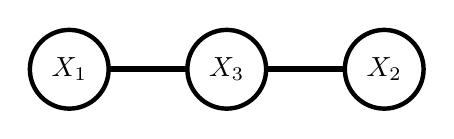
\begin{tikzpicture}[scale = 0.5]
\draw[black][fill=white,ultra thick](0,0)circle[radius=1];
\draw[black][fill=white,ultra thick](4,0)circle[radius=1];
\draw[black][fill=white,ultra thick](8,0)circle[radius=1];
\node at (0,0) [black][thick][scale=1]{$X_{1}$};
\node at (4,0) [black][thick][scale=1]{$X_{3}$};
\node at (8,0) [black][thick][scale=1]{$X_{2}$};
\draw [line width=2][-][black](1,0)--(3,0);
\draw [line width=2][-][black](5,0)--(7,0);
\end{tikzpicture}
\end{figure}

Problem b:
The inverse of $\Sigma$ contains no zero element, hence no conditional independency. Therefore there have to be edges between any two vertexes.
\begin{figure}[h]
\small
\centering
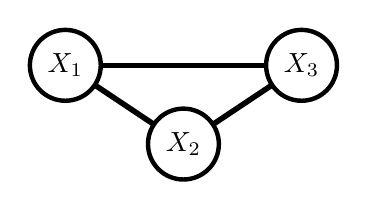
\begin{tikzpicture}[scale = 0.5]
\draw[black][fill=white,ultra thick](0,0)circle[radius=0.9];
\draw[black][fill=white,ultra thick](6,0)circle[radius=0.9];
\draw[black][fill=white,ultra thick](3,-2)circle[radius=0.9];
\node at (0,0) [black][thick][scale=1]{$X_{1}$};
\node at (6,0) [black][thick][scale=1]{$X_{3}$};
\node at (3,-2) [black][thick][scale=1]{$X_{2}$};
\draw [line width=2][-][black](0.75,-0.5)--(2.25,-1.5);
\draw [line width=2][-][black](5.25,-0.5)--(3.75,-1.5);
\draw [line width=2][-][black](0.9,0)--(5.1,0);
\end{tikzpicture}
\end{figure}

This model also cancels the marginal independency $X_{1}\perp X_{3}$. But it is possible to model this set of properties by Bayesian network with two directed edges $X_{1}\rightarrow X_{2}$ and $X_{3} \rightarrow X_{2}$. 

Problem c:
Consider the terms inside the exponential:
$$-\frac{1}{2}\left\{ x_{1}^{2} + (x_{2}-x_{1})^{2} + (x_{3}-x_{2}^{2}) \right\}$$

It is easy to see the precision matrix and covariance matrix take:
$$\Lambda=\begin{pmatrix}2 & -1 & 0 \\ -1 & 2 & -1 \\ 0 & -1 & 1\\ \end{pmatrix},\Sigma = \begin{pmatrix}1 & 1 & 1 \\ 1 & 2 & 2\\ 1 & 2 & 3\\ \end{pmatrix}$$

Problem d:
The only independency is $X_{1}\perp X_{3} | X_{2}$:
\begin{figure}[h]
\small
\centering
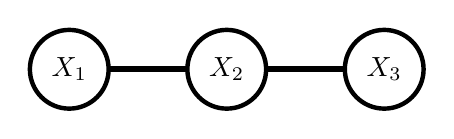
\begin{tikzpicture}[scale = 0.5]
\draw[black][fill=white,ultra thick](0,0)circle[radius=1];
\draw[black][fill=white,ultra thick](4,0)circle[radius=1];
\draw[black][fill=white,ultra thick](8,0)circle[radius=1];
\node at (0,0) [black][thick][scale=1]{$X_{1}$};
\node at (4,0) [black][thick][scale=1]{$X_{2}$};
\node at (8,0) [black][thick][scale=1]{$X_{3}$};
\draw [line width=2][-][black](1,0)--(3,0);
\draw [line width=2][-][black](5,0)--(7,0);
\end{tikzpicture}
\end{figure}

\subsection{Independencies in Gaussian graphical models}
Problem a and b:

This PGM implies $X_{1} \perp X_{3}|X_{2}$, hence we are looking for a precision matrix with $\Lambda_{1,3}=0$, thus C and D meet the condition. On the other hand, $(A^{-1})_{1,3}=(B^{-1})_{1,3}=0$. So A and B are candidates for covariance matrix.

Problem c and d:

This PGM tells that $X_{1} \perp X_{3}$. Hence C and D can be covariance matrix, A and B can be precision matrix. 

The only possible PGM is:
\begin{figure}[h]
\small
\centering
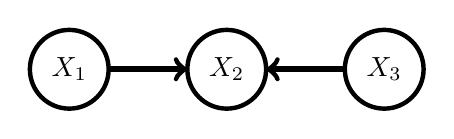
\begin{tikzpicture}[scale = 0.5]
\draw[black][fill=white,ultra thick](0,0)circle[radius=1];
\draw[black][fill=white,ultra thick](4,0)circle[radius=1];
\draw[black][fill=white,ultra thick](8,0)circle[radius=1];
\node at (0,0) [black][thick][scale=1]{$X_{1}$};
\node at (4,0) [black][thick][scale=1]{$X_{2}$};
\node at (8,0) [black][thick][scale=1]{$X_{3}$};
\draw [line width=2][->][black](1,0)--(3,0);
\draw [line width=2][<-][black](5,0)--(7,0);
\end{tikzpicture}
\end{figure}

Problem e:

The answer can be derived from the conclusion of marginal Gaussian directly, A is true while B not.

\subsection{Cost of training MRFs and CRFs}
The answer are generally:
$$O(r(Nc+1))$$

and
$$O(r(Nc+N))$$

\subsection{Full conditional in an Ising model}
Straightforwardly(we have omitted $\theta$ from condition w.l.o.g):
\begin{align}
p(x_{k}=1|\textbf{x}_{-k})=&\frac{p(x_{k}=1,\textbf{x}_{-k})}{p(\textbf{x}_{-k})} \nonumber \\
=&\frac{p(x_{k}=1,\textbf{x}_{-k})}{p(x_{k}=0,\textbf{x}_{-k})+p(x_{k}=1,\textbf{x}_{-k})} \nonumber \\
=&\frac{1}{1+\frac{p(x_{k}=0,\textbf{x}_{-k})}{p(x_{k}=1,\textbf{x}_{-k})}} \nonumber \\
=&\frac{1}{1+\frac{\exp(h_{k}\cdot 0)\prod_{<k,i>}\exp(J_{k,i}\cdot 0)}{\exp(h_{k}\cdot 1)\prod_{<k,i>}\exp(J_{k,i}\cdot x_{i})}} \nonumber \\
=&\sigma(h_{k}+\sum_{i=1,i\neq k}^{n}J_{k,i}x_{i}) \nonumber
\end{align}

When using denotation $x=\left\{ 0,1 \right\}$, the full conditional becomes:
$$p(x_{k}=1|\textbf{x}_{-k})\sigma(2\cdot (h_{k}+\sum_{i=1,i\neq k}^{n}J_{k,i}x_{i})) $$

\newpage
\section{Exact inference for graphical models}
\subsection{Variable elimination}
Where tf is the figure?!

\subsection{Gaussian times Gaussian is Gaussian}
We have:
\begin{align}
\ &N(x|\mu_{1},\lambda_{1}^{-1})\times N{N}(x|\mu_{2},\lambda_{2}^{-1})\nonumber \\
 =&\frac{\sqrt{\lambda_{1}\lambda_{2}}}{2\pi}\exp\left\{ -\frac{\lambda_{1}}{2}(x-\mu_{1})^{2}-\frac{\lambda_{2}}{2}(x-\mu_{2})^{2}  \right\}\nonumber \\
=& \frac{\sqrt{\lambda_{1}\lambda_{2}}}{2\pi} \exp\left\{ -\frac{\lambda_{1}+\lambda_{2}}{2}x^{2}+(\lambda_{1}\mu_{1}+\lambda_{2}\mu_{2})x-\frac{\lambda_{1}\mu_{1}^{2}+\lambda_{2}\mu_{2}^{2}}{2} \right\}  \nonumber
\end{align}

By completing the square:
\begin{align}
\ &\exp\left\{ -\frac{\lambda_{1}+\lambda_{2}}{2}x^{2}+(\lambda_{1}\mu_{1}+\lambda_{2}\mu_{2})x-\frac{\lambda_{1}\mu_{1}^{2}+\lambda_{2}\mu_{2}^{2}}{2} \right\} \nonumber \\
=&c\cdot \exp{-\frac{\lambda}{2}(x-\mu)^{2}}\nonumber
\end{align}

Where:
$$\lambda = \lambda_{1}+\lambda_{2}$$
$$\mu = \lambda^{-1}(\lambda_{1}\mu_{1}+\lambda_{2}\mu_{2})$$

The constant factor $c$ can be obtained by computing the constant terms inside the exponential.

\subsection{Message passing on a tree}
Problem a:

It is easy to see after variable elimination:
$$p(X_{2}=50) = \sum_{G_{1}}\sum_{G_{2}}p(G_{1})p(G_{2}|G_{1})p(X_{2}=50|G_{2})$$
$$p(G_{1}=1,X_{2}=50)=p(G_{1})\sum_{G_{2}}p(G_{2}|G_{1}=1)p(X_{2}=50|G_{2})$$

Thus:
$$p(G_{1}=1|X_{2}=50)=\frac{0.45+0.05\cdot \exp(-5)}{0.5 + 0.5 \cdot \exp(-5)}\approx 0.9$$

Problem b(here $X$ denotes $X_{2}$ or $X_{3}$):

\begin{align}
\ &p(G_{1}=1|X_{2}=50,X_{3}=50)\nonumber \\
 = &\frac{p(G_{1}=1,X_{2}=50,X_{3}=50)}{p(X_{2}=50,X_{3}=50)}\nonumber \\
=&\frac{p(G_{1}=1)p(X_{2}|G_{1}=1)p(X_{3}|G_{1}=1)}{p(G_{1}=0)p(X_{2}|G_{1}=0)p(X_{3}|G_{1}=0)+p(G_{1}=1)p(X_{2}|G_{1}=1)p(X_{3}|G_{1}=1)}\nonumber \\
=&\frac{p(X=50|G_{1}=1)^{2}}{p(X=50|G_{1}=0)^{2}+p(X=50|G_{1}=1)^{2}} \nonumber \\
\approx& \frac{0.9^{2}}{0.1^{2}+0.9^{2}} \approx 0.99 \nonumber
\end{align}

Extra evidence makes the belief in $G_{1}=1$ firmer.

Problem c:

The answer to problem c is symmetric to that to problem b, $p(G_{1}=0|X_{2}=60, X_{3}=60) \approx 0.99$.

Problem d:

Using the same pattern of analysis from Problem b, we have:
$$p(G_{1}=1|X_{2}=50, X_{3}=60)$$
$$=\frac{p(X=50|G_{1}=1)p(X=60|G_{1}=1)}{p(X=50|G_{1}=0)p(X=60|G_{1}=0)+p(X=50|G_{1}=1)p(X=60|G_{1}=1)}$$

Notice we have:
$$p(X=50|G_{1}=1)=p(X=60|G_{1}=0)$$
$$p(X=50|G_{1}=0)=p(X=60|G_{1}=1)$$

Hence:
$$P(G_{1}=1|X_{2}=50,X_{3}=60)=0.5$$

In this case, $X_{2}$ and $X_{3}$ have equal strength as evidence and their effects achieve a balance so they provide not enough information to distort the prior knowledge.

\subsection{Inference in 2D lattice MRFs}
Please refer to PGM:principals and techniques 11.4.1.


\newpage
\section{Variational inference}
\subsection{Laplace approximation to $p(\mu,\log \sigma|D)$ for a univariate Gaussian}
Laplace approximation equals representing $f(\mu,l)=\log p(\mu,l=\log \sigma|D)$ with second-order Taylor expansion. We have:
\begin{align}
\log p(\mu,l|D)=&\log p(\mu,l,D)-\log p(D)\nonumber \\
=&\log p(\mu,l) + \log p(D|\mu,l) + c \nonumber \\
=&\log p(D|\mu,l) + c \nonumber \\
=&\sum_{n=1}^{N}\log \frac{1}{\sqrt{2\pi\sigma^{2}}}\exp\left\{-\frac{1}{2\sigma^{2}}(y_{n}-\mu)^{2}  \right\}+c \nonumber \\
=&-N\log \sigma+\sum_{n=1}^{N}-\frac{1}{2\sigma^{2}}(y_{n}-\mu)^{2}+c\nonumber \\
=&-N\cdot l+\frac{1}{2}\frac{1}{\exp\left\{2\cdot l\right\}}\sum_{n=1}^{N}(y_{n}-\mu)^{2}+c \nonumber
\end{align}

Thus we derive:
\begin{align}
\frac{\partial \log p(\mu,l|D)}{\partial \mu}=&\frac{1}{2}\frac{1}{\exp\left\{2\cdot l\right\}}\sum_{n=1}^{N}2\cdot (y_{n}-\mu) \nonumber \\
=&\frac{N}{\sigma^{2}}\cdot (\bar{y}-\mu)\nonumber \\ 
\frac{\partial \log p(\mu,l|D)}{\partial l}=&-N + \frac{1}{2}\sum_{n=1}^{N}(y_{n}-\mu)^{2}\cdot (-2)\cdot \frac{1}{\exp\left\{2\cdot l  \right\}} \nonumber \\
=&-N+\frac{1}{\sigma^{2}}\sum_{n=1}^{N}(y_{n}-\mu)^{2} \nonumber \\
\frac{\partial^{2} \log p(\mu,l|D)}{\partial \mu^{2}}=&-\frac{N}{\sigma^{2}} \nonumber \\
\frac{\partial^{2} \log p(\mu,l|D)}{\partial l^{2}}=&-\frac{2}{\sigma^{2}}\sum_{n=1}^{N}(y_{n}-\mu)^{2} \nonumber \\
\frac{\partial^{2} \log p(\mu,l|D)}{\partial \mu \partial l}=&N\cdot (\bar{y}-\mu)\cdot (-2) \cdot \frac{1}{\sigma^{2}} \nonumber 
\end{align}

For approximation, $p(\mu,l) \approx N(\mu, \Sigma)$ with:
$$\Sigma = \begin{pmatrix} \frac{\partial^{2} \log p(\mu,l|D)}{\partial \mu^{2}} & \frac{\partial^{2} \log p(\mu,l|D)}{\partial l^{2}} \\ \frac{\partial^{2} \log p(\mu,l|D)}{\partial l^{2}} &  \frac{\partial^{2} \log p(\mu,l|D)}{\partial \mu \partial l} \\ \end{pmatrix}^{-1}$$
$$\mu = \Sigma \begin{pmatrix} \frac{\partial \log p(\mu,l|D)}{\partial \mu} \\ \frac{\partial \log p(\mu,l|D)}{\partial l}  \end{pmatrix}$$

\subsection{Laplace approximation to normal-gamma}
This is the same with exercise 21.1 when the prior is uniformative. We formally substitute:
\begin{align}
\sum_{n=1}^{N}(y_{n}-\mu)^{2}=& \sum_{n=1}^{N}((y_{n}-\bar{y})-(\mu-\bar{y}))^{2} \nonumber \\
=&\sum_{n=1}^{N}(y_{n}-\bar{y})^{2} + \sum_{n=1}^{N}(\mu-\bar{y})^{2} + 2(\mu-\bar{y})\cdot\sum_{n=1}^{N}(y_{n}-\bar{y})\nonumber \\
=&Ns^{2}+N(\mu-\bar{y})^{2} \nonumber
\end{align}

Where $s^{2}=\frac{1}{N}\sum_{n=1}^{N}(y_{n}-\bar{y})^{2}$

Conclusions in all problems a, b and c are included in the previous solution.

\subsection{Variational lower bound for VB for univariate Gaussian}
What left in section 21.5.1.6 is the derivation for 21.86 to 21.91. We omit the derivation for entropy for Gaussian and moments, which can be found in any information theory textbook. Now we derive the $\mathbb{E}[\ln x|x \sim Ga(a,b)]$, which can therefore yields to the entropy for a Gamma distribution.

We know that Gamma distribution is an exponential family distribution:
\begin{align}
Ga(x|a,b)=&\frac{b^{a}}{\Gamma(a)}x^{a-1}\exp\left\{-b\cdot x \right\}\nonumber \\
\propto& \exp\left\{-b\cdot x+(a-1) \ln x  \right\} \nonumber\\
=&\exp\left\{ \phi(x)^{T}\theta \right\}\nonumber
\end{align}

The sufficient statistics is $\phi(x)=(x,\ln x)^{T}$ and natural parameter is given by $\theta = (-b,a-1)^{T}$. Thus Gamma distribution can be seen as the maximum entropy distribution under constraints on $x$ and $\ln x$. 

The culumant function is given by:
\begin{align}
A(\theta)=& \log Z(\theta)\nonumber \\
=&\log \frac{\Gamma(a)}{b^{a}} \nonumber \\
=&\log \Gamma(a) - a \log b \nonumber
\end{align}

The expectation of sufficient statistics is given by the derivative of cumulant function, therefore:
$$\mathbb{E}[\ln x] = \frac{\partial A}{\partial (a-1)} = \frac{\Gamma'(a)}{\Gamma(a)}-\log b$$

According to defintion $\psi(a)=\frac{\Gamma'(a)}{\Gamma(a)}$:
$$\mathbb{E}[\ln x] = \psi(a)-\log b$$

The rest derivations are completed or trivial.

\subsection{Variational lower bound for VB for GMMs}
The lower bound is given by:
\begin{align}
\mathbb{E}_{q}[\log \frac{p(\theta,D)}{q(\theta)}] =& \mathbb{E}_{q}[\log p(\theta,D)] -\mathbb{E}_{q}[q(\theta)]\nonumber \\
=&\mathbb{E}_{q}[\log p(D|\theta)]+\mathbb{E}_{q}[\log p(\theta)]+\mathbb{E}_{q}[\log q(\theta)] \nonumber \\
=&\mathbb{E}[\log p(\textbf{x}|\textbf{z},\mu,\Lambda,\pi)] + \mathbb{E}[\log p(\textbf{z},\mu,\Lambda,\pi)]\nonumber \\
\ &-\mathbb{E}[\log q(\textbf{z},\mu,\Lambda,\pi)]\nonumber \\
=&\mathbb{E}[\log p(\textbf{x}|\textbf{z},\mu,\Lambda,\pi)] + \mathbb{E}[\log p(\textbf{z}|\pi)] + \mathbb{E}[\log p(\pi)] + \mathbb{E}[\log p(\mu, \Lambda)] \nonumber \\
\ &+ \mathbb{E}[\log q(\textbf{z})] + \mathbb{E}[\log q(\pi)] + \mathbb{E}[\log q(\mu,\Lambda)]\nonumber
\end{align}

We are now showing 21.209 to 21.215.

For 21.209:
\begin{align}
\mathbb{E}[\log p(\textbf{x}|\textbf{z},\mu,\Lambda)]=& \mathbb{E}_{q(\textbf{z})q(\mu,\Lambda)}[\log p(\textbf{x}|\textbf{z},\mu,\Lambda)] \nonumber \\
=& \sum_{n}\sum_{k}\mathbb{E}_{q(\textbf{z})q(\mu,\Lambda)}[-\frac{D}{2}\log 2\pi + \frac{1}{2}\log |\Lambda_{k}|-\frac{1}{2}(x_{n}-\mu_{k})^{T}\Lambda_{k}(x_{n}-\mu_{k})]\nonumber
\end{align}

Using 21.132 and converting summing by average $\bar{x}_{k}$ yields to solution.

For 21.210:
\begin{align}
\mathbb{E}[\log p(\textbf{z}|\pi)]=&\mathbb{E}_{q(\textbf{z})q(\pi)}[\log p(\textbf{z}|\pi)]\nonumber \\
=&\mathbb{E}_{q(\textbf{z})q(\pi)}[\log \prod_{n=1}^{N}\prod_{k=1}^{K}\pi_{k}^{z_{nk}}] \nonumber \\
=&\sum_{n=1}^{N}\sum_{k=1}^{K}\mathbb{E}_{q(\textbf{z})q(\pi)}[z_{nk}\log \pi_{k}]\nonumber \\
=&\sum_{n=1}^{N}\sum_{k=1}^{K}\mathbb{E}_{q(\textbf{z})}[z_{nk}]\mathbb{E}_{q(\pi)}[\log \pi_{k}]\nonumber \\
=&\sum_{n=1}^{N}\sum_{k=1}^{K}r_{nk}\log \bar{\pi}_{k}\nonumber
\end{align}

For 21.211:
\begin{align}
\mathbb{E}[\log p(\pi)]=&\mathbb{E}_{q(\pi)}[\log p(\pi)] \nonumber \\
=&\mathbb{E}_{q(\pi)}[\log (C\cdot \prod_{k=1}^{K}\pi_{k}^{\alpha_{0}-1})]\nonumber \\
=&\ln C + (\alpha_{0}-1)\sum_{k=1}^{K}\log \bar{\pi}_{k} \nonumber
\end{align}

For 21.212:
\begin{align}
\mathbb{E}[\log p(\mu,\Lambda)]=&\mathbb{E}_{q(\mu,\Lambda)}[\log p(\mu,\Lambda)] \nonumber \\
=&\mathbb{E}_{q(\mu,\Lambda)}[\log \prod_{k=1}^{K}Wi(\Lambda_{k}|L_{0},v_{0})\cdot N(\mu_{k}|m_{0},(\beta_{0}\Lambda_{k})^{-1}]\nonumber \\
=&\sum_{k=1}^{K}\mathbb{E}_{q(\mu,\Lambda)}[ \log C + \frac{1}{2}(v_{0}-D-1)\log |\Lambda_{k}| -\frac{1}{2}tr\left\{ \Lambda_{k}L_{0}^{-1} \right\}\nonumber \\
\ & - \frac{D}{2}\log 2 \pi - \frac{1}{2}\log |\beta_{0}\Lambda_{k}| -\frac{1}{2}(\mu_{k}-m_{0})^{T}(\beta_{0}\Lambda_{k})(\mu_{k}-m_{0}) ]\nonumber
\end{align}

Using 21.131 to expand the expected value of the quadratic form and using the fact that the mean of a Wi distribution is $v_{k}L_{k}$ and we are done.

For 21.213:
\begin{align}
\mathbb{E}[\log q(\textbf{z})]=& \mathbb{E}_{q(\textbf{z})}[\log q(\textbf{z})] \nonumber \\
=&\mathbb{E}_{q(\textbf{z})}[\sum_{i}\sum_{k}z_{ik}\log r_{ik}]\nonumber \\
=&\sum_{i}\sum_{k} \mathbb{E}_{q(\textbf{z})}[z_{ik}]\log r_{ik}\nonumber \\
=& \sum_{i}\sum_{k} r_{ik}\log r_{ik}\nonumber 
\end{align}

For 21.214:
\begin{align}
\mathbb{E}[\log q(\pi)]=&\mathbb{E}_{q(\pi)}[\log q(\pi)] \nonumber \\
=&\mathbb{E}_{q(\pi)}[\log C + \sum_{k=1}^{K}(\alpha_{k}-1)\log \pi_{k}] \nonumber \\
=&\log C + \sum_{k}(\alpha_{k}-1)\log \bar{\pi}_{k} \nonumber
\end{align}

For 21.215:
\begin{align}
\mathbb{E}[\log q(\mu,\Lambda)]=& \mathbb{E}_{q(\mu,\Lambda)}[\log q(\mu,\Lambda)] \nonumber \\
=&\sum_{k}\mathbb{E}_{q(\mu,\Lambda)}[\log q(\Lambda_{k})-\frac{D}{2}\log 2\pi +\frac{1}{2}\log |\beta_{k}\Lambda_{k}|\nonumber \\
\ &-\frac{1}{2}(\mu_{k}-m_{k})^{T}(\beta_{k}\Lambda_{k})(\mu_{k}-m_{k})  ]\nonumber 
\end{align}

Using 21.132 to expand the quadratic form to give $\mathbb{E}[(\mu_{k}-m_{k})^{T}(\beta_{k}\Lambda_{k})(\mu_{k}-m_{k})]=D$

\subsection{Derivation of $\mathbb{E}[\log \pi_{k}]$} under a Dirichlet distribution
Dirichlet distribution is an exponential family distribution, we have:
$$\phi(\pi)=(\log \pi_{1},\log \pi_{2},...\log \pi_{K})$$
$$\theta=\alpha$$

The cumulant function is:
$$A(\alpha)=\log B(\alpha) = \sum_{i=1}^{K}\log \Gamma(\alpha_{i})-\log \Gamma(\sum_{i=1}^{K}\alpha_{i})$$

And:
$$\mathbb{E}[\log \pi_{k}]=\frac{\partial A(\alpha)}{\partial \alpha_{k}} = \frac{\Gamma'(\alpha_{k})}{\Gamma(\alpha_{k})}- \frac{\Gamma'(\sum_{i=1}^{K}\alpha_{k})}{\Gamma(\sum_{i=1}^{K}\alpha_{k})}=\psi(\alpha_{k})-\psi(\sum_{i=1}^{K}\alpha_{i})$$

Take exponential on both sides:
$$\exp(\mathbb{E}[\log \pi_{k}])=\exp(\psi(\alpha_{k})-\psi(\sum_{i=1}^{K}\alpha_{k}))=\frac{\exp(\alpha_{k})}{\exp(\sum_{i=1}^{K}\alpha_{i})}$$

\subsection{Alternative derivation of the mean field updates for the Ising model}
This is no different than applying the procedure in section 21.3.1 before derivating updates, hence omitted.

\subsection{Forwards vs reverse KL divergence}
We have:
\begin{align}
KL(p(x,y)||q(x,y))=&\mathbb{E}_{p(x,y)}[\log \frac{p(x,y)}{q(x,y)}]\nonumber \\
=&\sum_{x,y}p(x,y)\log p(x,y)-\sum_{x,y}p(x,y)\log q(x)-\sum_{x,y}p(x,y)\log q(y) \nonumber \\
=&\sum_{x,y}p(x,y)\log p(x,y)-\sum_{x}(\sum_{y}p(x,y))\log q(x)-\sum{y}(\sum_{x}p(x,y))\log q(q) \nonumber \\
=&H(p(x,y))-H(p(x))-H(p(y))+KL(p(x)||q(x))+KL(p(y)||q(y))\nonumber \\
=& constant + KL(p(x)||q(x))+KL(p(y)||q(y))\nonumber
\end{align}

Thus the optimal approximation is $q(x)=p(x)$ and $q(y)=p(y)$.

We skip the practical part.

\subsection{Derivation of the structured mean field updates for FHMM}
According to the conclusion from mean-field varitional methods, we have:
$$E(\textbf{x}_{m})=\mathbb{E}_{q/m}[E(\bar{p}(\textbf{x}_{m}))]$$

Thus:
$$-\sum_{t=1}^{T}\sum_{k=1}^{K}x_{t,m,k}\tilde{\epsilon}_{t,m,k}=\frac{1}{2}\mathbb{E}[\sum_{t=1}^{T}(\textbf{y}_{t}-\sum_{l\neq m}^{M}W_{l}\textbf{x}_{t,m})^{T}\Sigma^{-1}(\textbf{y}_{t}-\sum_{l\neq m}^{M}W_{l}\textbf{x}_{t,m})]+C$$

Comparing the coefficient of $x_{t,m,k}$ (i.e. setting $x_{t,m,k}$ to 1) ends in:
$$\tilde{\epsilon}_{t,m,k}=W^{T}_{m}\Sigma^{-1}(\textbf{y}_{t}-\sum_{l\neq m}W_{l}\mathbb{E}[\textbf{x}_{t,l}])-\frac{1}{2}(W^{T}_{m}\Sigma^{-1}W_{m})_{k,k}$$

Write into matrix form yields to 21.62.

\subsection{Variational EM for binary FA with sigmoid link}
Refer to "Probabilistic Visualisation of High-Dimensional Binary Data, Tipping, 1998".

\subsection{VB for binary FA with probit link}
The major difference in using probit link is the uncontinuous likelihood caused by $p(y_{i}=1|z_{i})=\mathbb{I}(z_{i}>0)$. In the context of hiding $\textbf{X}$, we assume Gaussian prior on $\textbf{X}$, $\textbf{W}$ and $\textbf{Z}$. The approximation takes the form:
$$q(\textbf{X},\textbf{Z},\textbf{W})=\prod_{l=1}^{L}q(\textbf{w}_{l})\prod_{i=1}^{N}q(\textbf{x}_{i})q(z_{i})$$

It is a mean-field approximation, hence in an algorithm similari to EM, we are to update the distribution of $\textbf{X}$, $\textbf{Z}$ and $\textbf{W}$ stepwise.

For variable $\textbf{X}$, we have:
\begin{align}
\log q(\textbf{x}_{i})=&\mathbb{E}_{q(\textbf{z}_{i})q(\textbf{w})}[\log p(\textbf{x}_{i},\textbf{w},z_{i},y_{i})] \nonumber \\
=& \mathbb{E}_{q(\textbf{z}_{i})q(\textbf{w})}[\log p(\textbf{x}_{i})+\log p(\textbf{w})+\log p(z_{i}|\textbf{w}_{i},\textbf{w})+\log p(y_{i}|z_{i})] \nonumber
\end{align}

Given the likelihood form, for $i$ corresponding to $y_{i}=1$, $q(z_{i})$ have to be a truncated one, i.e. we only consider the expectations in the form $\mathbb{E}[z|z>\mu]$ and $\mathbb{E}[z^{2}|z>\mu]$.

$\log q(\textbf{x}_{i}) = -\frac{1}{2}\textbf{x}_{i}^{T}\Lambda_{1}\textbf{x}_{i}-\frac{1}{2}\mathbb{E}[z^{2}]-\frac{1}{2}\textbf{x}^{T}_{i} \mathbb{E}[\textbf{w}\textbf{w}^{T}]\textbf{x}_{i}+\mathbb{E}[z]\mathbb{E}[\textbf{w}]^{T}\textbf{x}_{i}$

Where $\Lambda_{1}$ is the covariance of $\textbf{x}_{i}$'s prior distribution, $\mathbb{E}[\textbf{w}\textbf{w}^{T}]$ can be calculated given the Gaussian form of $q(\textbf{w})$, and truncated expectations $\mathbb{E}[z]$ and $\mathbb{E}[z^{2}]$ can be obtained from solutions to exercise 11.15. It is obvious that $q(\textbf{x}_{i})$ is a Gaussian.

The update for $\textbf{w}$ is similar to that for $\textbf{x}_{i}$ as long as they play symmetric roles in likelihood. The only difference is we have to sum over $i$ when updating $\textbf{w}$.

At last we update $z_{i}$:
$$\log q(z_{i})=\mathbb{E}_{q(\textbf{x}_{i})q(\textbf{w})}[\log p(z_{i}|\textbf{x}_{i},\textbf{w})+\log p(y_{i}|z_{i})]$$

Inside the expectation we have:
$$-\frac{1}{2}z_{i}^{2}+\mathbb{E}[\textbf{w}]^{T}\mathbb{E}[\textbf{x}]z_{i}+c$$

Therefore $q(z_{i})$ again takes a Gaussian form.

\end{document}

%插入图片格式:
%\begin{figure}[h]
%\small
%\centering
%\includegraphics[width=6cm]{./gaussian/Maxwell_Laplace_Gaussian_.jpg}
%\caption{拉普拉斯近似,$\sigma^{2}=0.3$} \label{fig:aa}
%\end{figure}